\documentclass{beamer}
\usetheme[secheader]{Boadilla}
\usepackage{todonotes}
\defbeamertemplate*{footline}{Boadilla}
{
    \leavevmode%
    \hbox{%
%   \begin{beamercolorbox}[wd=.333333\paperwidth,ht=2.25ex,dp=1ex,right]{author in head/foot}%
%     \usebeamerfont{author in head/foot}\insertshortauthor~~(\insertshortinstitute)
%   \end{beamercolorbox}%
%   \begin{beamercolorbox}[wd=.333333\paperwidth,ht=2.25ex,dp=1ex,right]{title in head/foot}%
%     \usebeamerfont{title in head/foot}\insertshorttitle
%   \end{beamercolorbox}%
        \begin{beamercolorbox}[wd=1\paperwidth,ht=2.25ex,dp=1ex,right]{date in head/foot}%
%     \usebeamerfont{date in head/foot}\insertshortdate{}\hspace*{2em}
            \insertframenumber{}\hspace*{2ex}
        \end{beamercolorbox}}%
    \vskip0pt%
}

\usepackage{subfigure}



\usepackage{comment}
% wow this is a hack that lets you have more definitions in latex.
% see http://www.tex.ac.uk/cgi-bin/texfaq2html?label=noroom
\usepackage{natbib}
\usepackage{etex}
\usepackage{pgffor}
\usepackage[utf8]{inputenc}
%\usepackage[cyr]{aeguill}
%\reserveinserts{28}
\usepackage{tikz}
\usepackage[customcolors]{hf-tikz}
%\usepackage[utf8]{inputenc}
%\mode<presentation>{\usetheme{Caltech}}

\usepackage{amsmath}
\usepackage{mathtools}
\usepackage{amssymb}
\usepackage{amsfonts}
\usepackage{amsthm}
\usepackage{multimedia}
\usepackage{color}
\usepackage{esint}
\usepackage{stmaryrd}
\usepackage{tabularx}
\usepackage{multirow}
\usepackage[squaren]{SIunits}
\usepackage{graphicx}
\usepackage{diagbox}
\usepackage{pdfpages}
\usepackage{dsfont}
\usepackage{xcolor}
\usepackage{soul}
\usepackage[linesnumbered,ruled,vlined]{algorithm2e}


\graphicspath{{./img/}}

\newcommand{\cplus}{\colorbox{green}{($+$)} }
\newcommand{\cmoins}{\colorbox{red}{($-$)} }
\newcommand{\cmean}{\colorbox{yellow}{($\pm$)}}

\newcommand{\mathcolorbox}[2]{\colorbox{#1}{$\displaystyle #2$}}

%%%%% NEW MATH DEFINITIONS %%%%%

\usepackage{amsmath,amsfonts,bm}

% Mark sections of captions for referring to divisions of figures
\newcommand{\figleft}{{\em (Left)}}
\newcommand{\figcenter}{{\em (Center)}}
\newcommand{\figright}{{\em (Right)}}
\newcommand{\figtop}{{\em (Top)}}
\newcommand{\figbottom}{{\em (Bottom)}}
\newcommand{\captiona}{{\em (a)}}
\newcommand{\captionb}{{\em (b)}}
\newcommand{\captionc}{{\em (c)}}
\newcommand{\captiond}{{\em (d)}}

% Highlight a newly defined term
\newcommand{\newterm}[1]{{\bf #1}}


% Figure reference, lower-case.
\def\figref#1{figure~\ref{#1}}
% Figure reference, capital. For start of sentence
\def\Figref#1{Figure~\ref{#1}}
\def\twofigref#1#2{figures \ref{#1} and \ref{#2}}
\def\quadfigref#1#2#3#4{figures \ref{#1}, \ref{#2}, \ref{#3} and \ref{#4}}
% Section reference, lower-case.
\def\secref#1{section~\ref{#1}}
% Section reference, capital.
\def\Secref#1{Section~\ref{#1}}
% Reference to two sections.
\def\twosecrefs#1#2{sections \ref{#1} and \ref{#2}}
% Reference to three sections.
\def\secrefs#1#2#3{sections \ref{#1}, \ref{#2} and \ref{#3}}
% Reference to an equation, lower-case.
\def\eqref#1{equation~\ref{#1}}
% Reference to an equation, upper case
\def\Eqref#1{Equation~\ref{#1}}
% A raw reference to an equation---avoid using if possible
\def\plaineqref#1{\ref{#1}}
% Reference to a chapter, lower-case.
\def\chapref#1{chapter~\ref{#1}}
% Reference to an equation, upper case.
\def\Chapref#1{Chapter~\ref{#1}}
% Reference to a range of chapters
\def\rangechapref#1#2{chapters\ref{#1}--\ref{#2}}
% Reference to an algorithm, lower-case.
\def\algref#1{algorithm~\ref{#1}}
% Reference to an algorithm, upper case.
\def\Algref#1{Algorithm~\ref{#1}}
\def\twoalgref#1#2{algorithms \ref{#1} and \ref{#2}}
\def\Twoalgref#1#2{Algorithms \ref{#1} and \ref{#2}}
% Reference to a part, lower case
\def\partref#1{part~\ref{#1}}
% Reference to a part, upper case
\def\Partref#1{Part~\ref{#1}}
\def\twopartref#1#2{parts \ref{#1} and \ref{#2}}

\def\ceil#1{\lceil #1 \rceil}
\def\floor#1{\lfloor #1 \rfloor}
\def\1{\bm{1}}
\newcommand{\train}{\mathcal{D}}
\newcommand{\valid}{\mathcal{D_{\mathrm{valid}}}}
\newcommand{\test}{\mathcal{D_{\mathrm{test}}}}

\def\eps{{\epsilon}}


% Random variables
\def\reta{{\textnormal{$\eta$}}}
\def\ra{{\textnormal{a}}}
\def\rb{{\textnormal{b}}}
\def\rc{{\textnormal{c}}}
\def\rd{{\textnormal{d}}}
\def\re{{\textnormal{e}}}
\def\rf{{\textnormal{f}}}
\def\rg{{\textnormal{g}}}
\def\rh{{\textnormal{h}}}
\def\ri{{\textnormal{i}}}
\def\rj{{\textnormal{j}}}
\def\rk{{\textnormal{k}}}
\def\rl{{\textnormal{l}}}
% rm is already a command, just don't name any random variables m
\def\rn{{\textnormal{n}}}
\def\ro{{\textnormal{o}}}
\def\rp{{\textnormal{p}}}
\def\rq{{\textnormal{q}}}
\def\rr{{\textnormal{r}}}
\def\rs{{\textnormal{s}}}
\def\rt{{\textnormal{t}}}
\def\ru{{\textnormal{u}}}
\def\rv{{\textnormal{v}}}
\def\rw{{\textnormal{w}}}
\def\rx{{\textnormal{x}}}
\def\ry{{\textnormal{y}}}
\def\rz{{\textnormal{z}}}

% Random vectors
\def\rvepsilon{{\mathbf{\epsilon}}}
\def\rvtheta{{\mathbf{\theta}}}
\def\rva{{\mathbf{a}}}
\def\rvb{{\mathbf{b}}}
\def\rvc{{\mathbf{c}}}
\def\rvd{{\mathbf{d}}}
\def\rve{{\mathbf{e}}}
\def\rvf{{\mathbf{f}}}
\def\rvg{{\mathbf{g}}}
\def\rvh{{\mathbf{h}}}
\def\rvu{{\mathbf{i}}}
\def\rvj{{\mathbf{j}}}
\def\rvk{{\mathbf{k}}}
\def\rvl{{\mathbf{l}}}
\def\rvm{{\mathbf{m}}}
\def\rvn{{\mathbf{n}}}
\def\rvo{{\mathbf{o}}}
\def\rvp{{\mathbf{p}}}
\def\rvq{{\mathbf{q}}}
\def\rvr{{\mathbf{r}}}
\def\rvs{{\mathbf{s}}}
\def\rvt{{\mathbf{t}}}
\def\rvu{{\mathbf{u}}}
\def\rvv{{\mathbf{v}}}
\def\rvw{{\mathbf{w}}}
\def\rvx{{\mathbf{x}}}
\def\rvy{{\mathbf{y}}}
\def\rvz{{\mathbf{z}}}

% Elements of random vectors
\def\erva{{\textnormal{a}}}
\def\ervb{{\textnormal{b}}}
\def\ervc{{\textnormal{c}}}
\def\ervd{{\textnormal{d}}}
\def\erve{{\textnormal{e}}}
\def\ervf{{\textnormal{f}}}
\def\ervg{{\textnormal{g}}}
\def\ervh{{\textnormal{h}}}
\def\ervi{{\textnormal{i}}}
\def\ervj{{\textnormal{j}}}
\def\ervk{{\textnormal{k}}}
\def\ervl{{\textnormal{l}}}
\def\ervm{{\textnormal{m}}}
\def\ervn{{\textnormal{n}}}
\def\ervo{{\textnormal{o}}}
\def\ervp{{\textnormal{p}}}
\def\ervq{{\textnormal{q}}}
\def\ervr{{\textnormal{r}}}
\def\ervs{{\textnormal{s}}}
\def\ervt{{\textnormal{t}}}
\def\ervu{{\textnormal{u}}}
\def\ervv{{\textnormal{v}}}
\def\ervw{{\textnormal{w}}}
\def\ervx{{\textnormal{x}}}
\def\ervy{{\textnormal{y}}}
\def\ervz{{\textnormal{z}}}

% Random matrices
\def\rmA{{\mathbf{A}}}
\def\rmB{{\mathbf{B}}}
\def\rmC{{\mathbf{C}}}
\def\rmD{{\mathbf{D}}}
\def\rmE{{\mathbf{E}}}
\def\rmF{{\mathbf{F}}}
\def\rmG{{\mathbf{G}}}
\def\rmH{{\mathbf{H}}}
\def\rmI{{\mathbf{I}}}
\def\rmJ{{\mathbf{J}}}
\def\rmK{{\mathbf{K}}}
\def\rmL{{\mathbf{L}}}
\def\rmM{{\mathbf{M}}}
\def\rmN{{\mathbf{N}}}
\def\rmO{{\mathbf{O}}}
\def\rmP{{\mathbf{P}}}
\def\rmQ{{\mathbf{Q}}}
\def\rmR{{\mathbf{R}}}
\def\rmS{{\mathbf{S}}}
\def\rmT{{\mathbf{T}}}
\def\rmU{{\mathbf{U}}}
\def\rmV{{\mathbf{V}}}
\def\rmW{{\mathbf{W}}}
\def\rmX{{\mathbf{X}}}
\def\rmY{{\mathbf{Y}}}
\def\rmZ{{\mathbf{Z}}}

% Elements of random matrices
\def\ermA{{\textnormal{A}}}
\def\ermB{{\textnormal{B}}}
\def\ermC{{\textnormal{C}}}
\def\ermD{{\textnormal{D}}}
\def\ermE{{\textnormal{E}}}
\def\ermF{{\textnormal{F}}}
\def\ermG{{\textnormal{G}}}
\def\ermH{{\textnormal{H}}}
\def\ermI{{\textnormal{I}}}
\def\ermJ{{\textnormal{J}}}
\def\ermK{{\textnormal{K}}}
\def\ermL{{\textnormal{L}}}
\def\ermM{{\textnormal{M}}}
\def\ermN{{\textnormal{N}}}
\def\ermO{{\textnormal{O}}}
\def\ermP{{\textnormal{P}}}
\def\ermQ{{\textnormal{Q}}}
\def\ermR{{\textnormal{R}}}
\def\ermS{{\textnormal{S}}}
\def\ermT{{\textnormal{T}}}
\def\ermU{{\textnormal{U}}}
\def\ermV{{\textnormal{V}}}
\def\ermW{{\textnormal{W}}}
\def\ermX{{\textnormal{X}}}
\def\ermY{{\textnormal{Y}}}
\def\ermZ{{\textnormal{Z}}}

% Vectors
\def\vzero{{\bm{0}}}
\def\vone{{\bm{1}}}
\def\vmu{{\bm{\mu}}}
\def\vtheta{{\bm{\theta}}}
\def\va{{\bm{a}}}
\def\vb{{\bm{b}}}
\def\vc{{\bm{c}}}
\def\vd{{\bm{d}}}
\def\ve{{\bm{e}}}
\def\vf{{\bm{f}}}
\def\vg{{\bm{g}}}
\def\vh{{\bm{h}}}
\def\vi{{\bm{i}}}
\def\vj{{\bm{j}}}
\def\vk{{\bm{k}}}
\def\vl{{\bm{l}}}
\def\vm{{\bm{m}}}
\def\vn{{\bm{n}}}
\def\vo{{\bm{o}}}
\def\vp{{\bm{p}}}
\def\vq{{\bm{q}}}
\def\vr{{\bm{r}}}
\def\vs{{\bm{s}}}
\def\vt{{\bm{t}}}
\def\vu{{\bm{u}}}
\def\vv{{\bm{v}}}
\def\vw{{\bm{w}}}
\def\vx{{\bm{x}}}
\def\vy{{\bm{y}}}
\def\vz{{\bm{z}}}

% Elements of vectors
\def\evalpha{{\alpha}}
\def\evbeta{{\beta}}
\def\evepsilon{{\epsilon}}
\def\evlambda{{\lambda}}
\def\evomega{{\omega}}
\def\evmu{{\mu}}
\def\evpsi{{\psi}}
\def\evsigma{{\sigma}}
\def\evtheta{{\theta}}
\def\eva{{a}}
\def\evb{{b}}
\def\evc{{c}}
\def\evd{{d}}
\def\eve{{e}}
\def\evf{{f}}
\def\evg{{g}}
\def\evh{{h}}
\def\evi{{i}}
\def\evj{{j}}
\def\evk{{k}}
\def\evl{{l}}
\def\evm{{m}}
\def\evn{{n}}
\def\evo{{o}}
\def\evp{{p}}
\def\evq{{q}}
\def\evr{{r}}
\def\evs{{s}}
\def\evt{{t}}
\def\evu{{u}}
\def\evv{{v}}
\def\evw{{w}}
\def\evx{{x}}
\def\evy{{y}}
\def\evz{{z}}

% Matrix
\def\mA{{\bm{A}}}
\def\mB{{\bm{B}}}
\def\mC{{\bm{C}}}
\def\mD{{\bm{D}}}
\def\mE{{\bm{E}}}
\def\mF{{\bm{F}}}
\def\mG{{\bm{G}}}
\def\mH{{\bm{H}}}
\def\mI{{\bm{I}}}
\def\mJ{{\bm{J}}}
\def\mK{{\bm{K}}}
\def\mL{{\bm{L}}}
\def\mM{{\bm{M}}}
\def\mN{{\bm{N}}}
\def\mO{{\bm{O}}}
\def\mP{{\bm{P}}}
\def\mQ{{\bm{Q}}}
\def\mR{{\bm{R}}}
\def\mS{{\bm{S}}}
\def\mT{{\bm{T}}}
\def\mU{{\bm{U}}}
\def\mV{{\bm{V}}}
\def\mW{{\bm{W}}}
\def\mX{{\bm{X}}}
\def\mY{{\bm{Y}}}
\def\mZ{{\bm{Z}}}
\def\mBeta{{\bm{\beta}}}
\def\mPhi{{\bm{\Phi}}}
\def\mLambda{{\bm{\Lambda}}}
\def\mSigma{{\bm{\Sigma}}}

% Tensor
\DeclareMathAlphabet{\mathsfit}{\encodingdefault}{\sfdefault}{m}{sl}
\SetMathAlphabet{\mathsfit}{bold}{\encodingdefault}{\sfdefault}{bx}{n}
\newcommand{\tens}[1]{\bm{\mathsfit{#1}}}
\def\tA{{\tens{A}}}
\def\tB{{\tens{B}}}
\def\tC{{\tens{C}}}
\def\tD{{\tens{D}}}
\def\tE{{\tens{E}}}
\def\tF{{\tens{F}}}
\def\tG{{\tens{G}}}
\def\tH{{\tens{H}}}
\def\tI{{\tens{I}}}
\def\tJ{{\tens{J}}}
\def\tK{{\tens{K}}}
\def\tL{{\tens{L}}}
\def\tM{{\tens{M}}}
\def\tN{{\tens{N}}}
\def\tO{{\tens{O}}}
\def\tP{{\tens{P}}}
\def\tQ{{\tens{Q}}}
\def\tR{{\tens{R}}}
\def\tS{{\tens{S}}}
\def\tT{{\tens{T}}}
\def\tU{{\tens{U}}}
\def\tV{{\tens{V}}}
\def\tW{{\tens{W}}}
\def\tX{{\tens{X}}}
\def\tY{{\tens{Y}}}
\def\tZ{{\tens{Z}}}


% Graph
\def\gA{{\mathcal{A}}}
\def\gB{{\mathcal{B}}}
\def\gC{{\mathcal{C}}}
\def\gD{{\mathcal{D}}}
\def\gE{{\mathcal{E}}}
\def\gF{{\mathcal{F}}}
\def\gG{{\mathcal{G}}}
\def\gH{{\mathcal{H}}}
\def\gI{{\mathcal{I}}}
\def\gJ{{\mathcal{J}}}
\def\gK{{\mathcal{K}}}
\def\gL{{\mathcal{L}}}
\def\gM{{\mathcal{M}}}
\def\gN{{\mathcal{N}}}
\def\gO{{\mathcal{O}}}
\def\gP{{\mathcal{P}}}
\def\gQ{{\mathcal{Q}}}
\def\gR{{\mathcal{R}}}
\def\gS{{\mathcal{S}}}
\def\gT{{\mathcal{T}}}
\def\gU{{\mathcal{U}}}
\def\gV{{\mathcal{V}}}
\def\gW{{\mathcal{W}}}
\def\gX{{\mathcal{X}}}
\def\gY{{\mathcal{Y}}}
\def\gZ{{\mathcal{Z}}}

% Sets
\def\sA{{\mathbb{A}}}
\def\sB{{\mathbb{B}}}
\def\sC{{\mathbb{C}}}
\def\sD{{\mathbb{D}}}
% Don't use a set called E, because this would be the same as our symbol
% for expectation.
\def\sF{{\mathbb{F}}}
\def\sG{{\mathbb{G}}}
\def\sH{{\mathbb{H}}}
\def\sI{{\mathbb{I}}}
\def\sJ{{\mathbb{J}}}
\def\sK{{\mathbb{K}}}
\def\sL{{\mathbb{L}}}
\def\sM{{\mathbb{M}}}
\def\sN{{\mathbb{N}}}
\def\sO{{\mathbb{O}}}
\def\sP{{\mathbb{P}}}
\def\sQ{{\mathbb{Q}}}
\def\sR{{\mathbb{R}}}
\def\sS{{\mathbb{S}}}
\def\sT{{\mathbb{T}}}
\def\sU{{\mathbb{U}}}
\def\sV{{\mathbb{V}}}
\def\sW{{\mathbb{W}}}
\def\sX{{\mathbb{X}}}
\def\sY{{\mathbb{Y}}}
\def\sZ{{\mathbb{Z}}}

% Entries of a matrix
\def\emLambda{{\Lambda}}
\def\emA{{A}}
\def\emB{{B}}
\def\emC{{C}}
\def\emD{{D}}
\def\emE{{E}}
\def\emF{{F}}
\def\emG{{G}}
\def\emH{{H}}
\def\emI{{I}}
\def\emJ{{J}}
\def\emK{{K}}
\def\emL{{L}}
\def\emM{{M}}
\def\emN{{N}}
\def\emO{{O}}
\def\emP{{P}}
\def\emQ{{Q}}
\def\emR{{R}}
\def\emS{{S}}
\def\emT{{T}}
\def\emU{{U}}
\def\emV{{V}}
\def\emW{{W}}
\def\emX{{X}}
\def\emY{{Y}}
\def\emZ{{Z}}
\def\emSigma{{\Sigma}}

% entries of a tensor
% Same font as tensor, without \bm wrapper
\newcommand{\etens}[1]{\mathsfit{#1}}
\def\etLambda{{\etens{\Lambda}}}
\def\etA{{\etens{A}}}
\def\etB{{\etens{B}}}
\def\etC{{\etens{C}}}
\def\etD{{\etens{D}}}
\def\etE{{\etens{E}}}
\def\etF{{\etens{F}}}
\def\etG{{\etens{G}}}
\def\etH{{\etens{H}}}
\def\etI{{\etens{I}}}
\def\etJ{{\etens{J}}}
\def\etK{{\etens{K}}}
\def\etL{{\etens{L}}}
\def\etM{{\etens{M}}}
\def\etN{{\etens{N}}}
\def\etO{{\etens{O}}}
\def\etP{{\etens{P}}}
\def\etQ{{\etens{Q}}}
\def\etR{{\etens{R}}}
\def\etS{{\etens{S}}}
\def\etT{{\etens{T}}}
\def\etU{{\etens{U}}}
\def\etV{{\etens{V}}}
\def\etW{{\etens{W}}}
\def\etX{{\etens{X}}}
\def\etY{{\etens{Y}}}
\def\etZ{{\etens{Z}}}

% The true underlying data generating distribution
\newcommand{\pdata}{p_{\rm{data}}}
% The empirical distribution defined by the training set
\newcommand{\ptrain}{\hat{p}_{\rm{data}}}
\newcommand{\Ptrain}{\hat{P}_{\rm{data}}}
% The model distribution
\newcommand{\pmodel}{p_{\rm{model}}}
\newcommand{\Pmodel}{P_{\rm{model}}}
\newcommand{\ptildemodel}{\tilde{p}_{\rm{model}}}
% Stochastic autoencoder distributions
\newcommand{\pencode}{p_{\rm{encoder}}}
\newcommand{\pdecode}{p_{\rm{decoder}}}
\newcommand{\precons}{p_{\rm{reconstruct}}}

\newcommand{\laplace}{\mathrm{Laplace}} % Laplace distribution

\newcommand{\E}{\mathbb{E}}
\newcommand{\Ls}{\mathcal{L}}
\newcommand{\R}{\mathbb{R}}
\newcommand{\emp}{\tilde{p}}
\newcommand{\lr}{\alpha}
\newcommand{\reg}{\lambda}
\newcommand{\rect}{\mathrm{rectifier}}
\newcommand{\softmax}{\mathrm{softmax}}
\newcommand{\sigmoid}{\sigma}
\newcommand{\softplus}{\zeta}
\newcommand{\KL}{D_{\mathrm{KL}}}
\newcommand{\Var}{\mathrm{Var}}
\newcommand{\standarderror}{\mathrm{SE}}
\newcommand{\Cov}{\mathrm{Cov}}
% Wolfram Mathworld says $L^2$ is for function spaces and $\ell^2$ is for vectors
% But then they seem to use $L^2$ for vectors throughout the site, and so does
% wikipedia.
\newcommand{\normlzero}{L^0}
\newcommand{\normlone}{L^1}
\newcommand{\normltwo}{L^2}
\newcommand{\normlp}{L^p}
\newcommand{\normmax}{L^\infty}

\newcommand{\parents}{Pa} % See usage in notation.tex. Chosen to match Daphne's book.

\DeclareMathOperator*{\argmax}{arg\,max}
\DeclareMathOperator*{\argmin}{arg\,min}

\DeclareMathOperator{\sign}{sign}
\DeclareMathOperator{\Tr}{Tr}
\let\ab\allowbreak

%\input{../glossary.tex}
\newcommand{\Q}{Q}
\newcommand{\V}{V}
\newcommand{\mubot}{\mu_{\bot}}
\newcommand{\mutop}{\mu_{\top}}
\newcommand{\params}{\theta}
\newcommand{\dirac}{\delta}
\newcommand{\normal}{\mathcal{N}}
\newcommand{\binomial}{\mathcal{B}}
\newcommand{\features}{\phi}
\newcommand{\maxiteration}{K}
\newcommand{\deltastoppingcriterion}{\upsilon}
\newcommand{\extrasmallvalue}{\kappa}
\newcommand{\egreedy}{\epsilon}
\newcommand{\users}{\rU}
\newcommand{\timeslot}{\tau}
\newcommand{\cooperationrate}{\varrho}
\newcommand{\T}{N}
\newcommand{\srs}{\nu}
\newcommand{\ser}{\xi}
\newcommand{\transpose}{\top}
\newcommand{\indextransition}{i}
\newcommand{\state}{s}
\newcommand{\n}{k}
\newcommand{\learningrate}{\alpha}
\newcommand{\abo}{\overline{\mathcal{T}}}
\newcommand{\bo}{\mathcal{T}}
\newcommand{\oQ}{\overline{Q}}
\newcommand{\Qr}{Q_r}
\newcommand{\Qc}{Q_c}
\newcommand{\oR}{\overline{R}}
\newcommand{\oV}{\overline{V}}
\newcommand{\Vr}{V_r}
\newcommand{\Vc}{V_c}
\newcommand{\ocS}{\overline{\mathcal{S}}}
\newcommand{\ocA}{\overline{\mathcal{A}}}
\newcommand{\cS}{\mathcal{S}}
\newcommand{\budgetspace}{\mathscr{B}}
\newcommand{\cK}{\mathcal{K}}
\newcommand{\policies}{\overline{\Pi}}
\newcommand{\cU}{\mathcal{U}}
\newcommand{\cA}{\mathcal{A}}
\newcommand{\augmentedtransition}{\overline{P}}
\newcommand{\cD}{\mathcal{D}}
\newcommand{\reward}{R}
\newcommand{\augmentedreward}{\overline{R}}
\newcommand{\constraint}{C}
\newcommand{\transition}{P}
\newcommand{\return}{G}
\newcommand{\constraintreturn}{G_c}
\newcommand{\augmentedreturn}{\overline{G}}
\newcommand{\cM}{\mathcal{M}}
\newcommand{\policy}{\pi}
\newcommand{\budgetedpolicy}{\overline{\pi}}
\newcommand{\optimalpolicy}{\pi^*}
\newcommand{\optimalbudgetedpolicy}{\overline{\pi}^*}
\newcommand{\discountfactor}{\gamma}
\newcommand{\budgetaction}{\beta_a}
\newcommand{\nextbudget}{\beta'}
\newcommand{\budget}{\beta}
\newcommand{\projection}{\Xi}
\newcommand{\augmentedprojection}{\overline{\Xi}}

\beamertemplatenavigationsymbolsempty

\author[shortname]{Nicolas Carrara}
\institute[shortinst]{University of Toronto}

\title[ROMA]{ROMA: Multi-Agent RL with Emergent Roles}
\subtitle{Tonghan Wang, Heng Dong, Victor Lesser and Chongjie Zhang}

\date{April 15, 2020}
\begin{document}
    \begin{frame}
        \maketitle
        \centering
    \end{frame}

    \begin{frame}{Cooperative \textbf{M}ulti \textbf{A}gent \textbf{R}einforcement \textbf{L}earning}

        \begin{figure}
            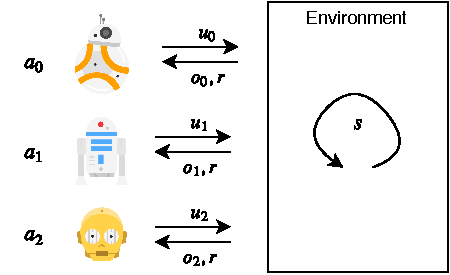
\includegraphics[width=0.75\linewidth]{img/marl.pdf}
            %\caption{Comparison of our method against baseline algorithms. Results for more maps can be found in Appendix C.1.}\label{fig:performance-baselines}
        \end{figure}
        \pause
        \begin{exampleblock}{}
            Can be cast as a Dec-POMDP
        \end{exampleblock}

    \end{frame}

    \begin{frame}{\textbf{Dec}entralized \textbf{P}artially \textbf{O}bservable \textbf{M}arkov \textbf{D}ecision \textbf{P}rocess}


        \begin{columns}
            \pause
            \begin{column}{0.45\textwidth}
                \begin{block}{Definition}
                    $G=\left\langle S,U,P,r,Z,O,n,\gamma\right\rangle$
                    \begin{itemize}
                        \item[$n$] the number of agents.
                        \item[$S$] the true-state space.
                        \item[$U$] the joint action space.
                        \item[$P$] the transition function.
                        \item[$r$] the reward function.
                        \item[$Z$] the observation space.
                        \item[$O$] the observation function.
                        \item[$\gamma$] the discount factor.
                    \end{itemize}
                \end{block}
            \end{column}
            \pause
            \begin{column}{0.50\textwidth}
                \begin{block}{Solving a Dec-POMDP}
                    \begin{itemize}
                        \item[$\tau^a$] action-observation history.
                        \item[$\pi^a$] the stochastic local policy
                        \item[$\pi$] the stochastic joint policy.
                        \item[$R_t$] $=\sum^{\infty}_{i=0}\gamma^ir_{t+i}$ the return.
                    \end{itemize}
                \end{block}
            \end{column}
        \end{columns}

    \end{frame}

    \begin{frame}{Two extremes solutions}
        \pause
        \begin{block}{Cast as an MDP.}
            \begin{itemize}
                \item[] \cplus Optimal solution.
                \item[] \cmoins Action space untractable.
                \item[] \cmoins Assume the agents can transmit their observations to a global controller.
                %\item Q-learning, DQN, IMPALA ...
            \end{itemize}
        \end{block}
        \pause
        \begin{block}{Several local MDPs.}
            \begin{itemize}
                \item[] \cplus Tractable.
                \item[] \cplus Local views.
                \item[] \cmoins Not optimal.
                \item[] \cmoins May not converge (non stationarity).
                %\item IQL ...
            \end{itemize}
        \end{block}
    \end{frame}

    \begin{frame}{Mixing architectures}

        Based on \textbf{C}entralized \textbf{T}raining \textbf{D}ecentralized \textbf{E}xecution.

        \begin{columns}
            \pause
            \begin{column}{0.5\textwidth}
                \begin{figure}
                    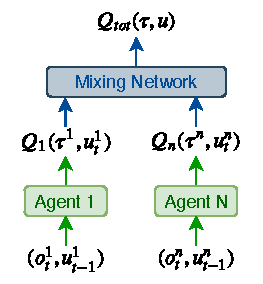
\includegraphics[width=\linewidth]{img/mixing_network.pdf}
                    %\caption{Comparison of our method against baseline algorithms. Results for more maps can be found in Appendix C.1.}\label{fig:performance-baselines}
                \end{figure}
            \end{column}
            \pause
            \begin{column}{0.5\textwidth}  %%<--- here
                \begin{block}{Example}
                    \textbf{V}alue \textbf{D}ecomposition \textbf{N}etworks.

                    \begin{equation}
                        Q_{tot}(\boldsymbol{\tau}, \mathbf{u}) = \sum_{i=1}^n Q_i (\tau^i, u^i;\theta^i)\nonumber.
                    \end{equation}
                \end{block}
            \end{column}
        \end{columns}

    \end{frame}

    \begin{frame}{Q-mix}
        \vspace{-0.5cm}
        \begin{columns}
            \pause
            \begin{column}{0.62\textwidth}
                \begin{block}{Generalisation of $Q_{tot}$ factorisation.}
                    \begin{equation}
                        \argmax_{\mathbf{u}}Q_{tot}(\boldsymbol{\tau}, \mathbf{u}) =
                        \begin{pmatrix}
                            \argmax_{u^1}Q_1(\tau^1, u^1)   \\
                            \vdots \\
                            \argmax_{u^n}Q_n(\tau^n, u^n) \\
                        \end{pmatrix}\nonumber
                    \end{equation}
                \end{block}
            \end{column}
            \pause
            \begin{column}{0.33\textwidth}  %%<--- here
                \begin{minipage}[c][0.5\textheight][c]{\linewidth}
                    \begin{block}{Enforcing monotonicity}
                        \begin{equation}
                            \frac{\partial Q_{tot}}{\partial Q_a}  \geq 0,~ \forall a \in A. \nonumber
                        \end{equation}
                    \end{block}
                \end{minipage}
            \end{column}
        \end{columns}

        \pause
        \begin{center}
            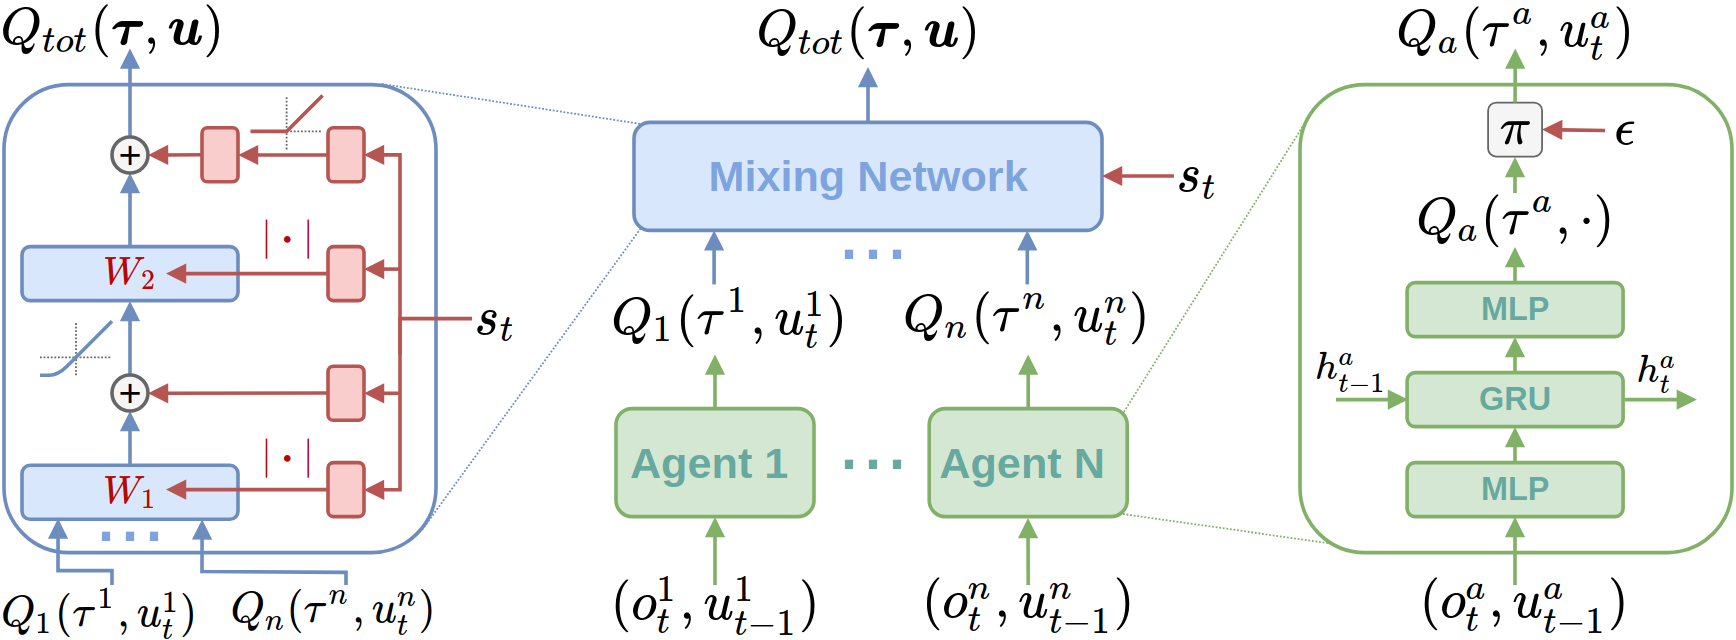
\includegraphics[width=0.75\linewidth]{img/QMIX.png}
        \end{center}


    \end{frame}

    \begin{frame}{ROMA}

        \pause
        \begin{alertblock}{Limit}
            Mixing architectures are not sufficient for complex tasks with subtasks.
        \end{alertblock}
        \pause
        \begin{exampleblock}{Solution:  \textbf{R}ole \textbf{O}riented \textbf{M}ulti-\textbf{A}gents RL.}
            Define and assign roles/skills to agents.
            \begin{itemize}
                \item[$\rightarrow$] Construction of a stochastic role embedding space.
            \end{itemize}
        \end{exampleblock}

    \end{frame}

    \begin{frame}{The space}
        \begin{figure}
            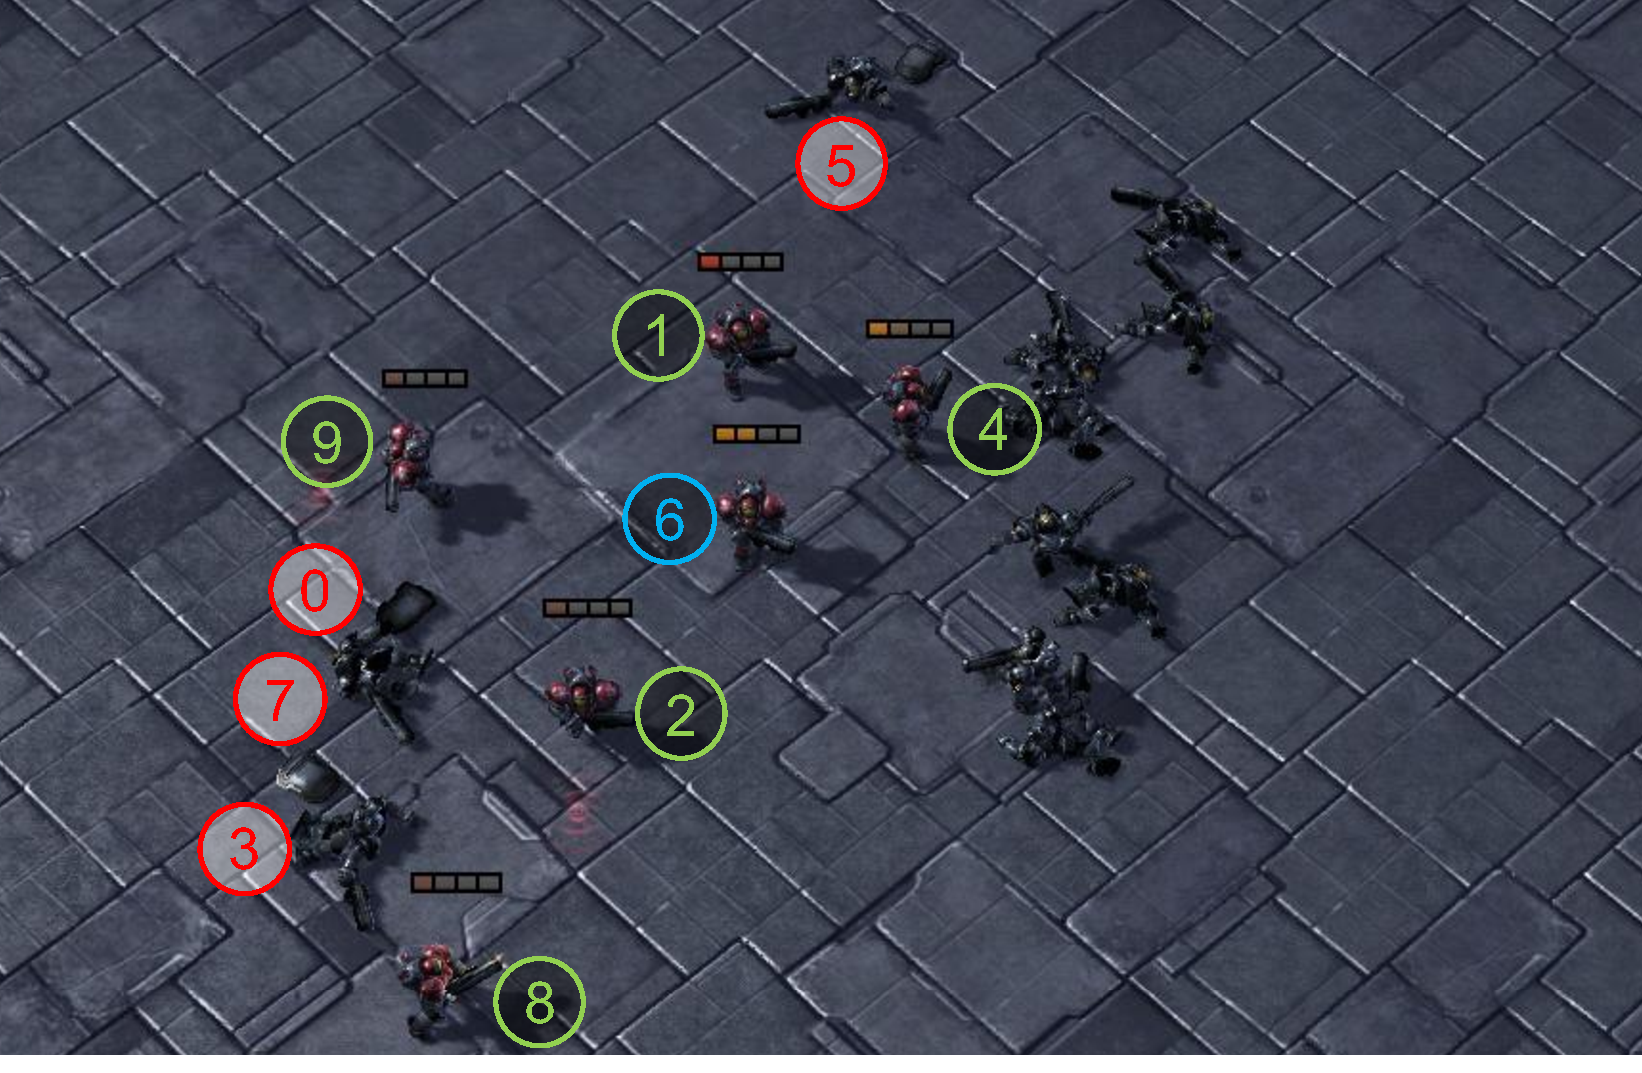
\includegraphics[height=0.35\linewidth]{img/10m_vs_11m-g4.pdf}\hfill
            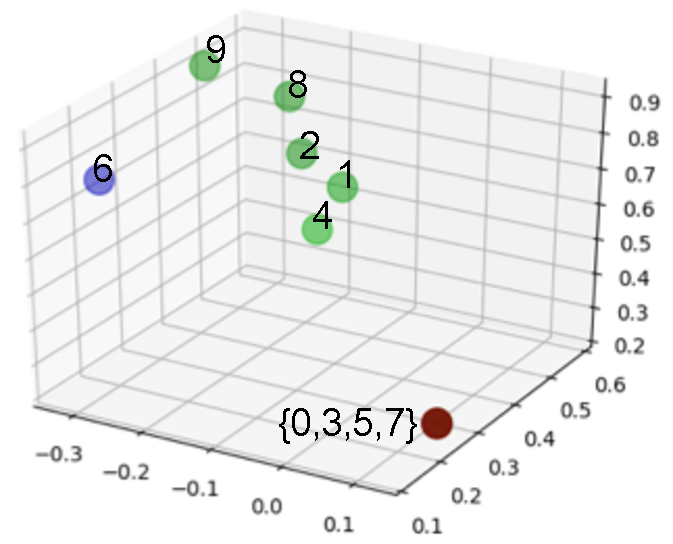
\includegraphics[height=0.35\linewidth]{img/10m_vs_11m-r4.pdf}\hfill
            %\caption{Visualization of our learned role representations at a timestep.
            %The blue agent has the maximum health, while the red ones are dead.
            %The corresponding policy is that agent 6 moves towards enemies to take on more firepower,
            %so that more seriously injured agents are protected.
            %Roles can change adaptively and will aggregate according to responsibilities that are compatible
            %with individual characteristics, such as location, agent type, health, etc.}\label{fig:teaser}
        \end{figure}
        \pause
        \begin{block}{}
            How to construct this space? Through regularizations of the loss function.
        \end{block}
    \end{frame}

    \begin{frame}{Some notations}

        % TODO maybe put a vienne diagram

        \begin{itemize}
            \item $i$: agent $i$.
            \item $\mathcal{L}$: a loss.
            \item $H(X)$: entropy.
            \item $\mathcal{CE}(X\|Y)$: cross-entropy
            \item $I(X;Y)$: mutual Information.
            \item $I(X;Y|Z)$ conditional mutual information.

        \end{itemize}

    \end{frame}

    \begin{frame}{The loss function}
        To define the loss, those roles properties must be fullfield:

        \begin{itemize}
            \item Dynamic;
            \item Versatile;
            \item Identifiable;
            \item Specialized.
        \end{itemize}
    \end{frame}

    \begin{frame}{Dynamic}
        Two complementary aspects:

        \begin{itemize}
            \item Roles encoding in a stochastic embedding space.
            \begin{itemize}
                \item $\rho_i \sim \normal(\mu_{\rho_i},\sigma_{\rho_i})$
            \end{itemize}
            \item Role are dictacted by a local observation.
            \begin{itemize}
                \item $(\mu_{\rho_i},\sigma_{\rho_i}) = f(o_i|\theta_{\rho})$
            \end{itemize}
        \end{itemize}

    \end{frame}

    \begin{frame}{Identifiable and versatile ($\mathcal{L}_{I}$)}

        \begin{itemize}
            \item Versatility: given an observation, roles should be diverse.
            \begin{itemize}
                \item Maximize $\mathcolorbox{yellow}{H(\rho_i|o_i)}$
            \end{itemize}
            \pause\item Identifiability: a trajectory (behavior) must be identifiable by a role.
            \begin{itemize}
                \item Minimize $\mathcolorbox{yellow}{H(\rho_i|\tau_i, o_i)}$
            \end{itemize}
        \end{itemize}
        \pause
        \begin{exampleblock}{Solution}
            maximize $\mathcolorbox{yellow}{I(\tau_i;\rho_i|o_i)}$.
        \end{exampleblock}
%        \pause
%        \begin{block}{In other words}
%            For a given agent and an observation, we enforce a bijection between roles and trajectories.
%        \end{block}
        \pause
        \begin{alertblock}{Limits}
            Untractable.
        \end{alertblock}
    \end{frame}
    \begin{frame}{Identifiable and versatile ($\mathcal{L}_{I}$)}

        \begin{exampleblock}{Solution (\colorbox{green}{variational posterior estimator $q_\xi$})}

            $\mathcal{L}_I(\theta_\rho, \xi) = \mathbb{E}_{(\tau^{t-1}_i, o^t_i)\sim D}\big[\mathcal{CE}[p(\rho^{t}_i | o^t_i)\| \mathcolorbox{green}{q_\xi(\rho^{t}_i | \tau^{t-1}_i, o^t_i)}] - H(\rho^{t}_i | o^t_i)\big]$

        \end{exampleblock}

%        \todo{(talk about $q_\eta$ ?)}
        \pause
        \begin{block}{}
            But what about roles \textbf{across} agents ?
        \end{block}

    \end{frame}

    \begin{frame}{Specialization ($\mathcal{L}_{D}$)}
        To encourage subtasks specialization:
        \pause
        % and thus can share their experiences to improve performances
        \begin{exampleblock}{Solution}
            Maximize $\mathcolorbox {yellow}{I(\rho_i;\tau_j| o_j)}$
        \end{exampleblock}
        \pause
        \begin{alertblock}{Limit}
            All agents will have the same role (and policy)
        \end{alertblock}
    \end{frame}
%    \begin{frame}{Specialization ($\mathcal{L}_{D}$)}
%        \begin{exampleblock}{Solution (disimilarity model)}
%            Maximize $I(\rho_i;\tau_j) + \mathcolorbox {green}{d_{\phi}(\tau_i,\tau_j)}$
%        \end{exampleblock}
%        \pause
%        \begin{alertblock}{Limit}
%            Might discard $d_{\phi}$
%        \end{alertblock}
%    \end{frame}
    \begin{frame}{Specialization ($\mathcal{L}_{D}$)}

        To encourage subtasks specialization:

        \begin{exampleblock}{Solution (dissimilarity and constrained program)}

            \begin{align*}
                & \text{Let}\ {D_\phi=(d_{\phi}(\tau_i,\tau_j))_{i,j}}\\
                &\mathcolorbox{orange}{\underset{{\theta_\rho, \xi, \phi}}{\text{minimize}}} \ \ \ \mathcolorbox {orange}{\|D_\phi^t\|_{0}} \\
                &\text{subject to} \ \ \ \mathcolorbox {yellow}{I(\rho^{t}_i; \tau^{t-1}_j|o^t_j)} + \mathcolorbox {orange}{d_\phi(\tau^{t-1}_i, \tau^{t-1}_j)} \mathcolorbox {yellow}{>U}, \forall i\ne j
            \end{align*}

%
        \end{exampleblock}

%        where $U$ controls the compactness of the embedding space.
        \pause
        \begin{block}{}
            Encourage \colorbox{yellow}{compactness} and \colorbox{orange}{diversity} ($U$ is the slider).
        \end{block}
        \pause
        \begin{alertblock}{Limit}
            Untractable
        \end{alertblock}
    \end{frame}

    \begin{frame}{Specialization ($\mathcal{L}_{D}$)}
        \begin{exampleblock}{Solution (\colorbox{cyan}{relaxation} and \colorbox{green}{variational posterior estimator})}
            \begin{align*}
                &\mathcal{L}_D(\theta_\rho, \phi, \xi) =
                \\ &\mathbb{E}_{(\bm{\tau}^{t-1}, \bm{o}^t)\sim\mathcal{D}, \bm{\rho}^t\sim p(\bm{\rho}^t | \bm{o}^t)}
                \\ &\big[\|D_\phi^t\|_{\mathcolorbox{cyan}{F}} - \sum_{i\ne j}\min\{\mathcolorbox{green}{q_\xi(\rho^{t}_i| \tau^{t-1}_j, o^t_j)} + d_\phi(\tau^{t-1}_i, \tau^{t-1}_j), U\}\big]
            \end{align*}
        \end{exampleblock}

    \end{frame}


    \begin{frame}{Including roles in the mixing architecture.}

        At each step:
        \begin{itemize}
            \pause\item Observation is encoded into role distribution parameters.
            \pause\item A role is sampled.
            \pause\item The role is decoded through an hypernet $\mathcolorbox{yellow}{g_{\theta_h}}$ then feed to the local utility network.
        \end{itemize}

    \end{frame}

%    \begin{exampleblock}{Solution}
%        Learn a dissimilarity model $d_{\phi}$ for trajectories:
%        \begin{itemize}
%            \item Maximise $I(\rho_i;\tau_j) + d_{\phi}(\tau_i,\tau_j)$
%        \end{itemize}
%    \end{exampleblock}

    \begin{frame}{Putting things togetheir}

        If $\theta=(\theta_\rho, \xi, \phi, \theta_h, \theta_m)$, $\lambda_I$ and $\lambda_D$ are scaling factors.

        \only<1>{
            \begin{block}{Final loss}
                $\mathcal{L}(\theta)= \mathcal{L}_{TD}(\theta)
                + \lambda_{I} \mathcal{L}_{I}(\theta_{\rho},\xi)
                + \lambda_{D}\mathcal{L}_{D}(\theta_{\rho},\xi,\phi)$\\
            \end{block}
            \begin{itemize}
                \item[] {}
            \end{itemize}
        }

        \only<2>{
            \begin{block}{Final loss}
                $\mathcal{L}(\theta)= \mathcolorbox {green}{\mathcal{L}_{TD}(\theta_m)}
                + \lambda_{I} \mathcal{L}_{I}(\theta_{\rho},\xi)
                + \lambda_{D}\mathcal{L}_{D}(\theta_{\rho},\xi,\phi)$
            \end{block}

            \begin{itemize}
                \item Temporal Difference loss \\$\mathcal{L}_{TD}(\theta_m)$ = $[r + \gamma \max_{\va'} Q_{tot}(s', \bm{a'}; \theta_m^-)$-$Q_{tot}$($s, \bm{a}; \theta_m$)$]^2$.
            \end{itemize}
        }
        \only<3>{
            \begin{block}{Final loss}
                $\mathcal{L}(\theta)= \mathcal{L}_{TD}(\theta_m)
                + \lambda_{I} \mathcolorbox {green}{\mathcal{L}_{I}(\theta_{\rho},\xi)}
                + \lambda_{D}\mathcal{L}_{D}(\theta_{\rho},\xi,\phi)$
            \end{block}

            \begin{itemize}
                \item Identifiability and versatility loss.
            \end{itemize}
        }
        \only<4>{
            \begin{block}{Final loss}
                $\mathcal{L}(\theta)= \mathcal{L}_{TD}(\theta_m)
                + \lambda_{I} \mathcal{L}_{I}(\theta_{\rho},\xi)
                + \lambda_{D}\mathcolorbox {green}{\mathcal{L}_{D}(\theta_{\rho},\xi,\phi)}$
            \end{block}

            \begin{itemize}
                \item Specialization loss.
            \end{itemize}
        }
    \end{frame}

    \begin{frame}{The framework}

        \begin{figure}
            \centering
            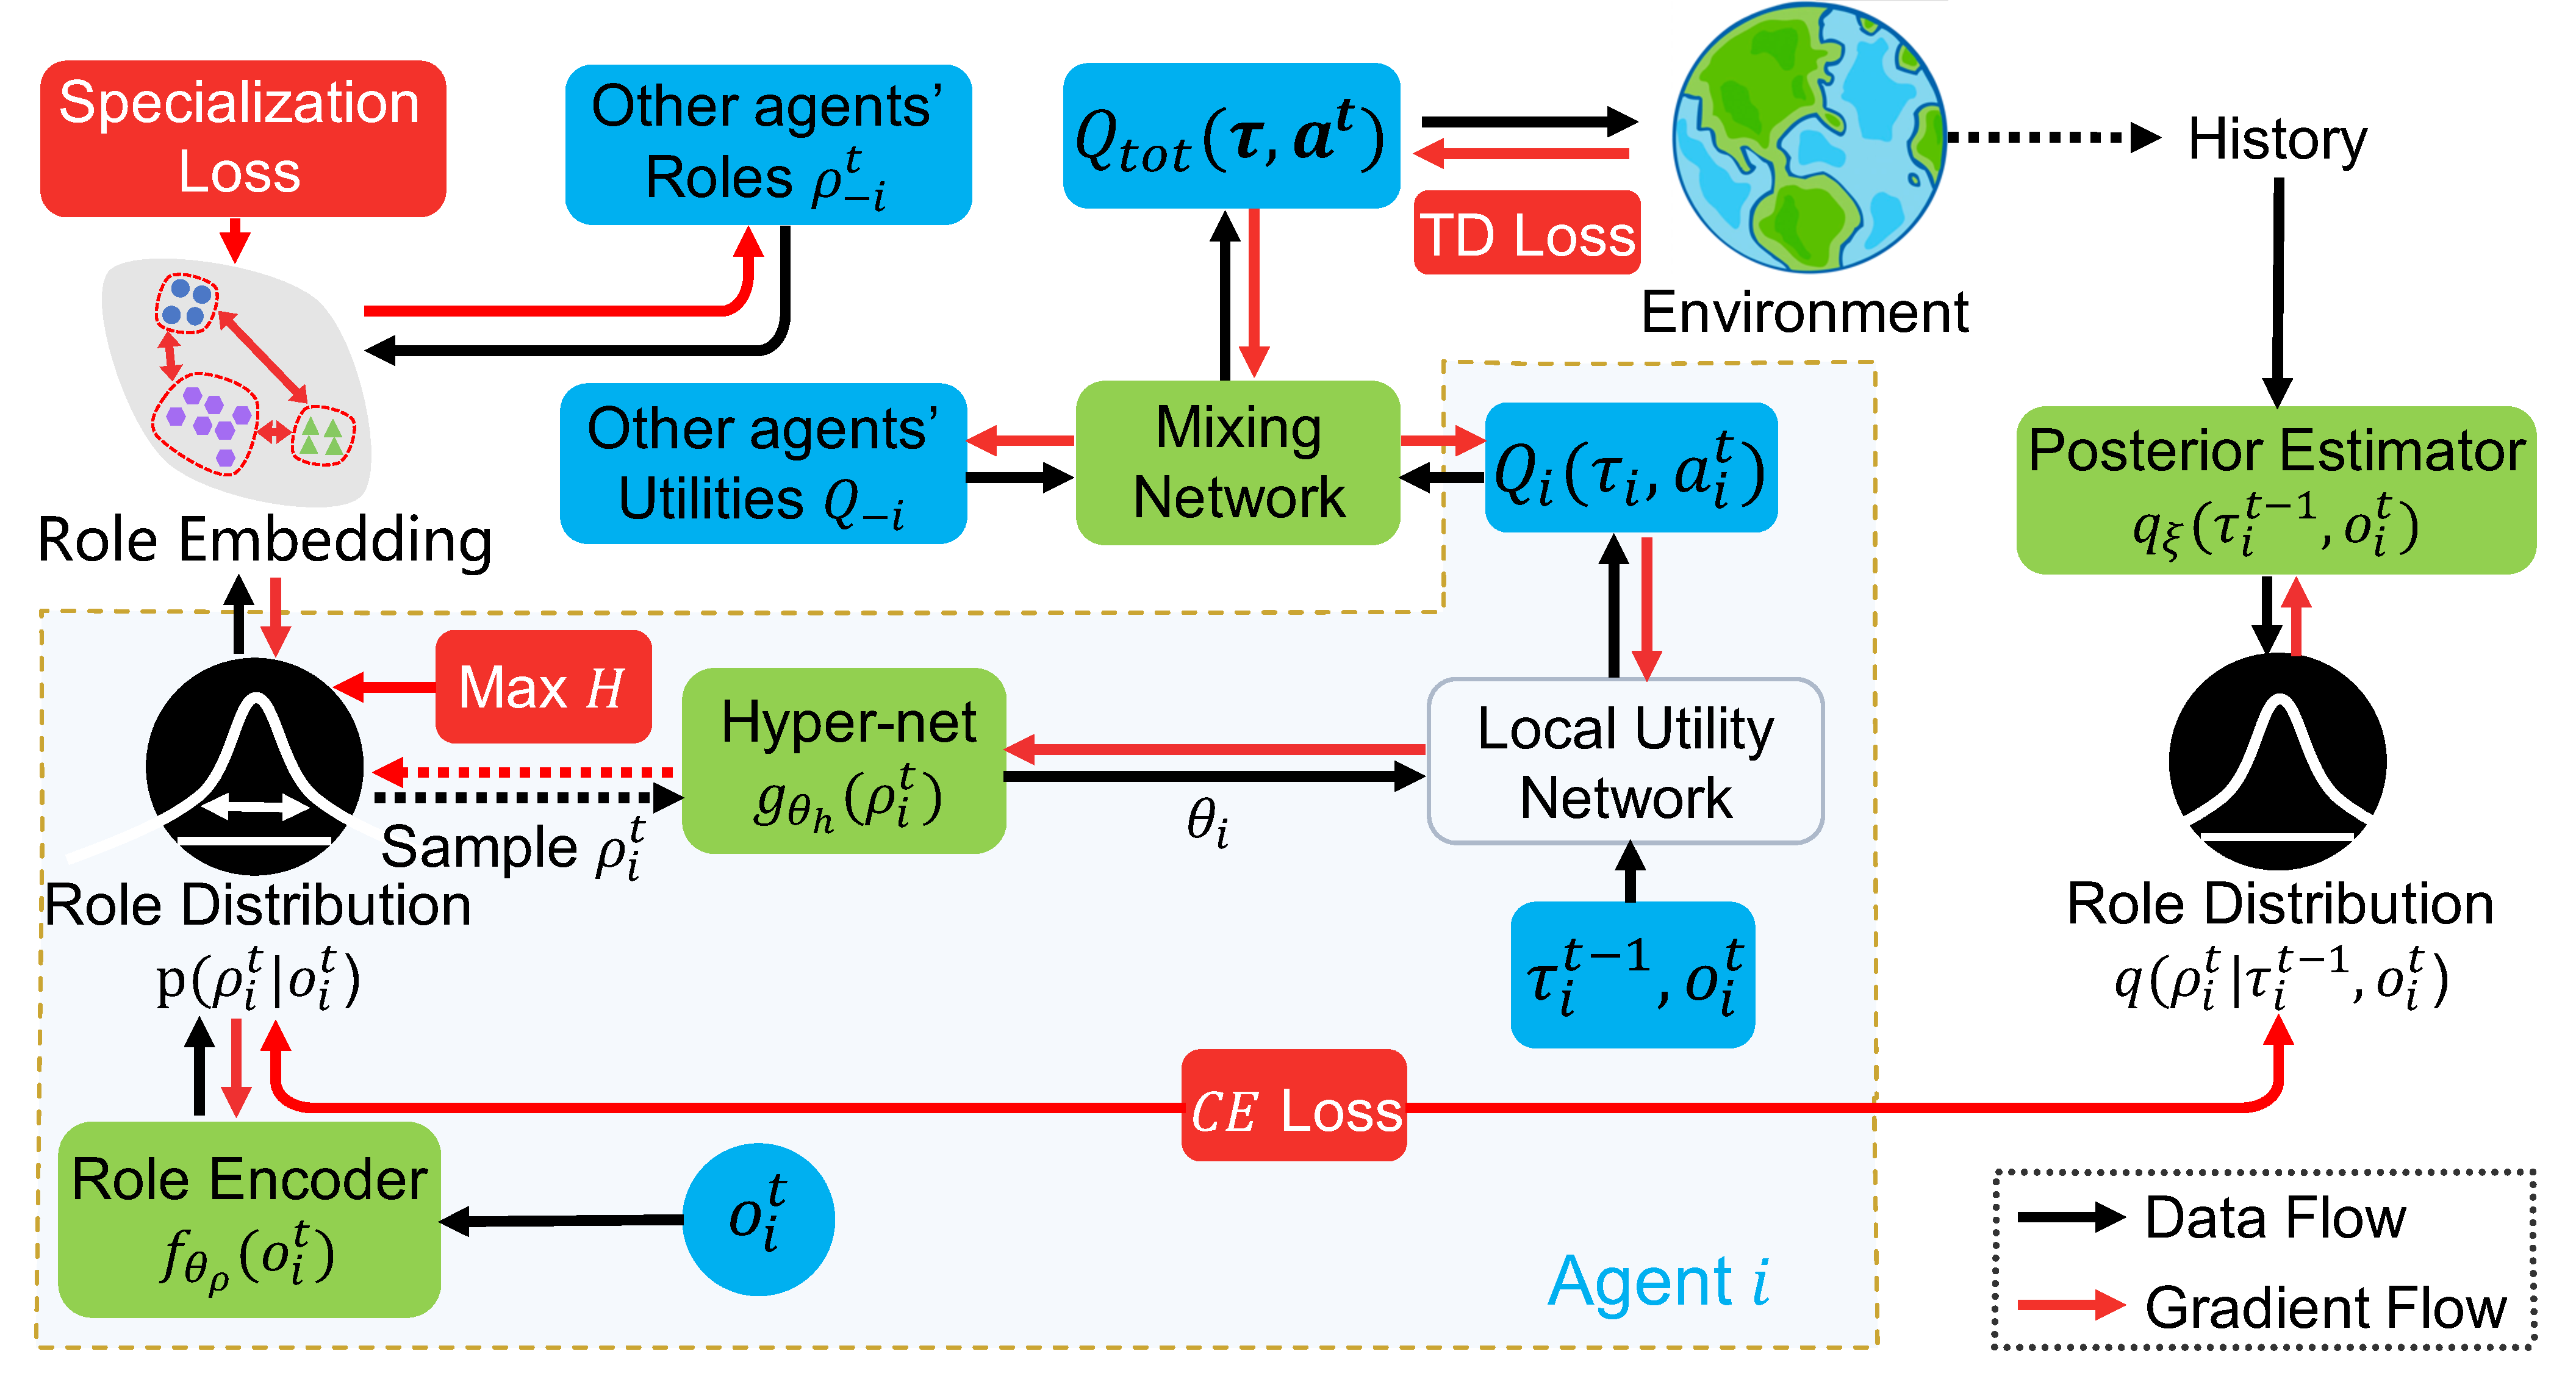
\includegraphics[width=1\linewidth]{img/framework.pdf}
            %\caption{Schematics of our approach. The role encoder generates a role embedding distribution, from which a role is sampled and serves as an input to the hyper-net. The hyper-net generates the parameters of the local utility network. Local utilities are fed into a mixing network to get an estimation of the global action value. During the interactions with other agents and the environment, individual trajectories are collected and fed into the trajectory encoder to get posterior estimations of the role distributions. The framework can be trained in an end-to-end fashion.}
            %\label{fig:framework}
        \end{figure}


    \end{frame}

    \begin{frame}{Some results}

        \begin{figure}
            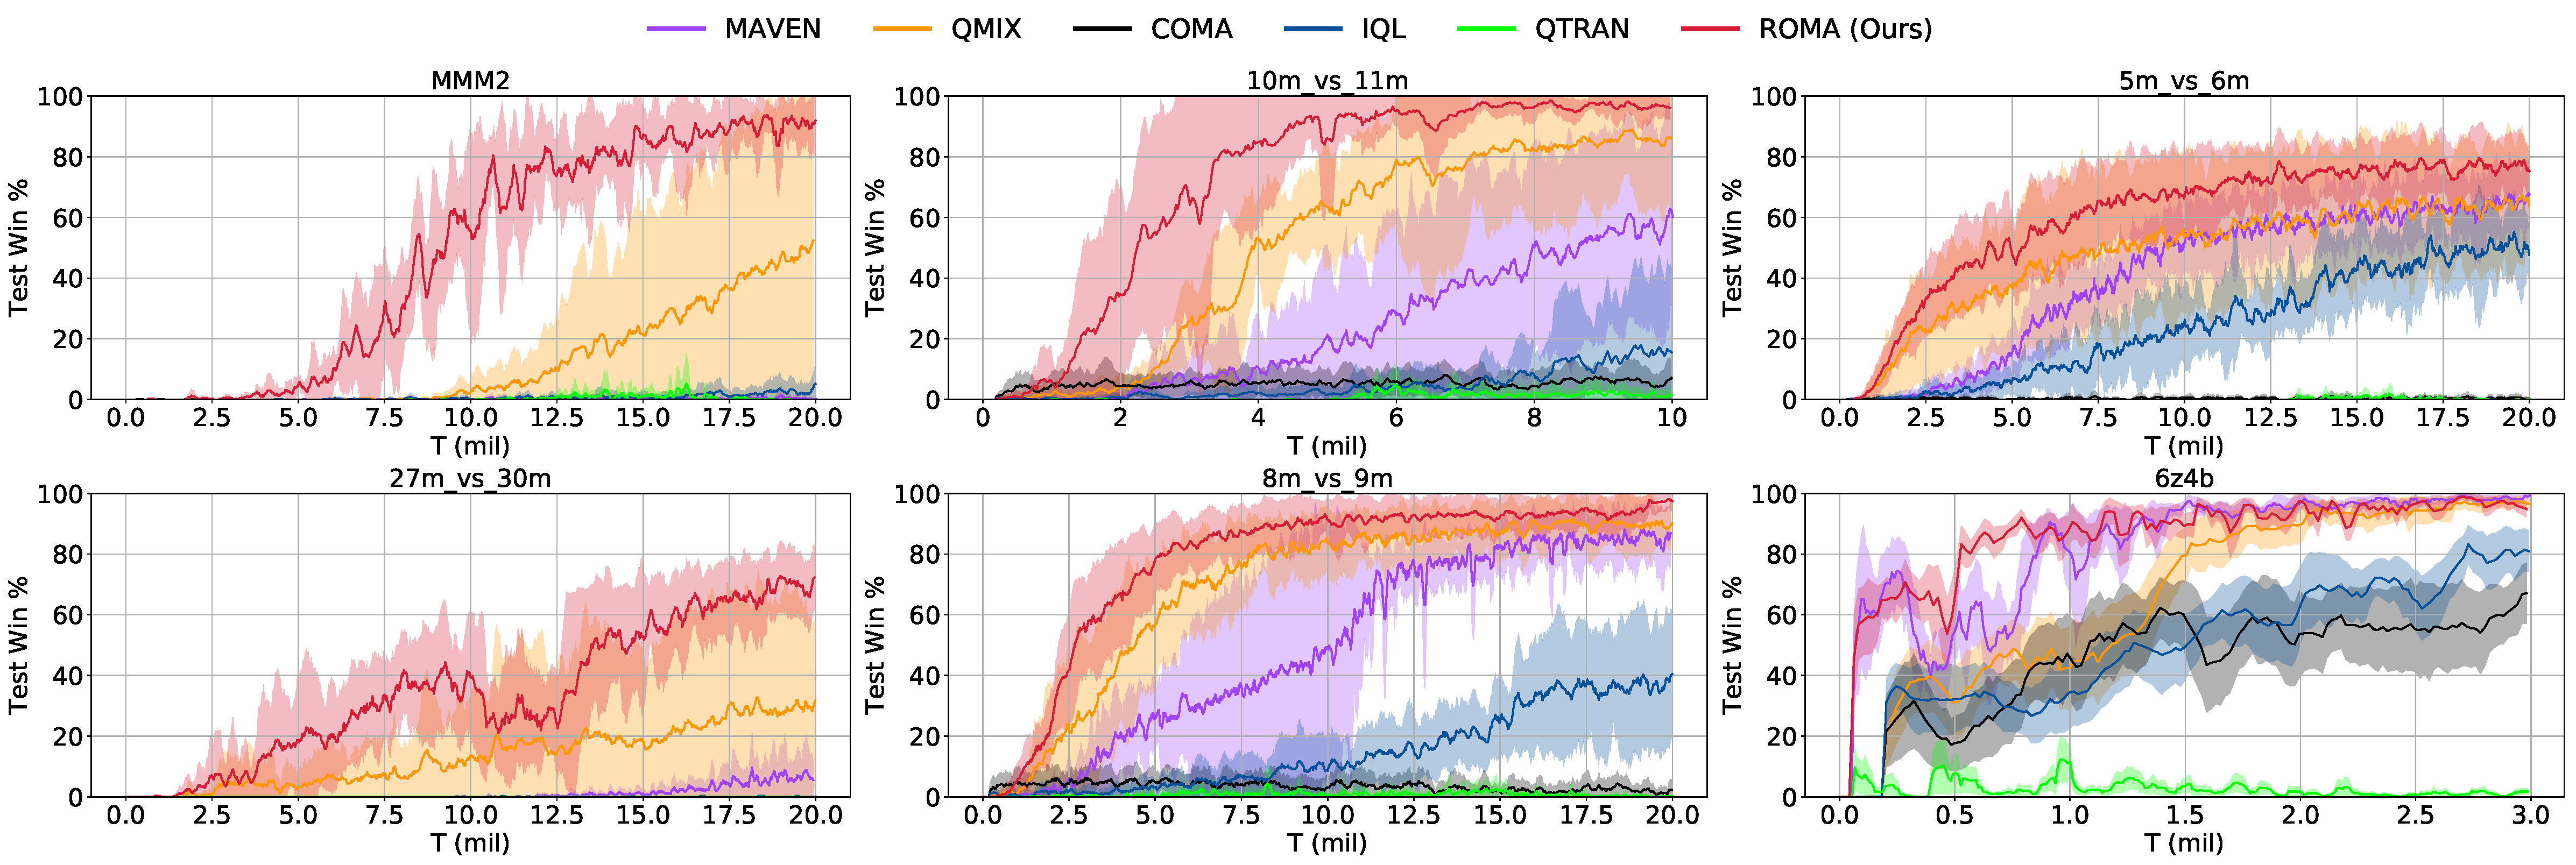
\includegraphics[width=\linewidth]{img/fig-lc/learning_curve.pdf}
            %\caption{Comparison of our method against baseline algorithms. Results for more maps can be found in Appendix C.1.}\label{fig:performance-baselines}
        \end{figure}
        \pause
        \begin{figure}
            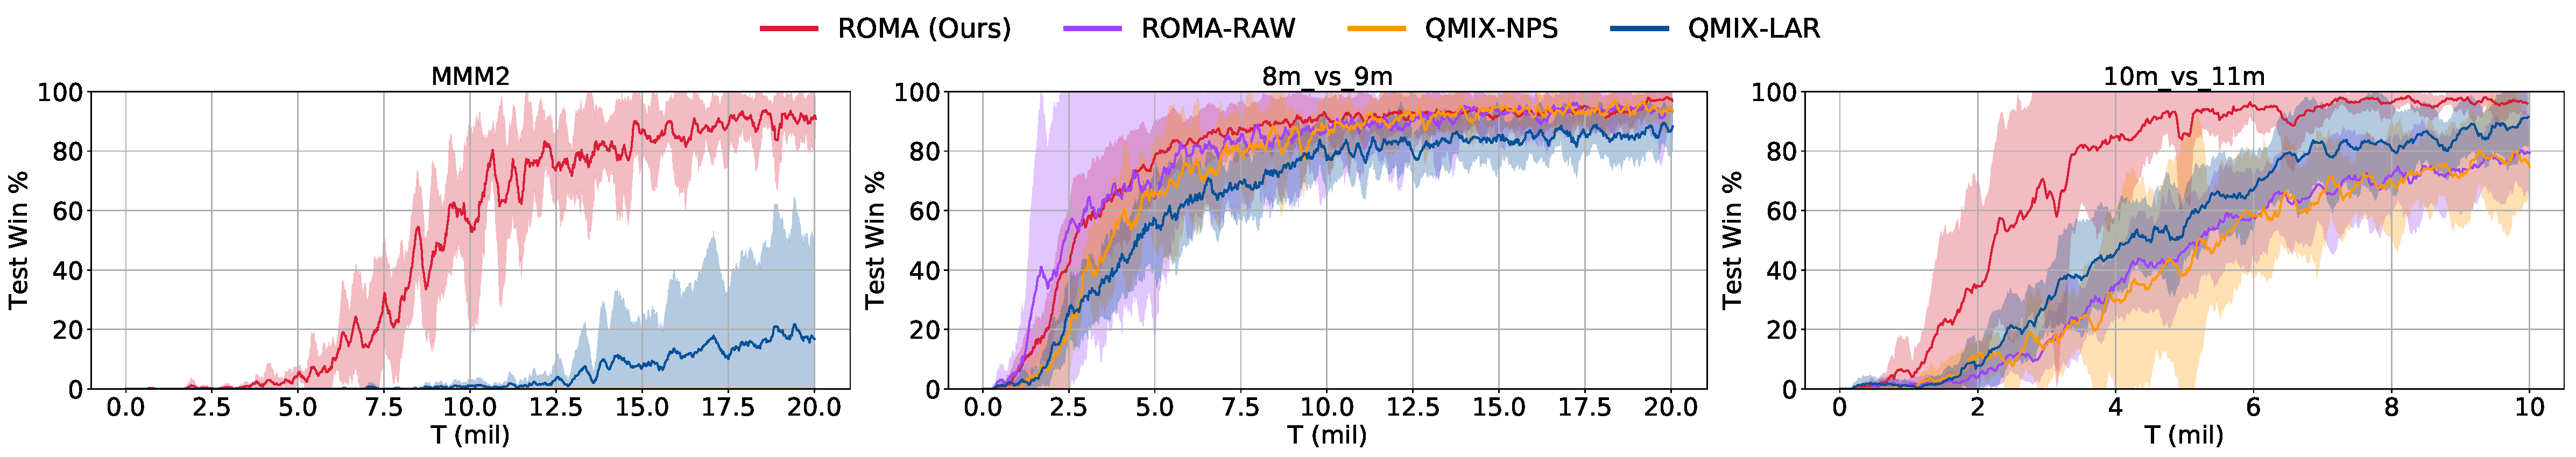
\includegraphics[width=\linewidth]{img/fig-lc/ablation.pdf}
            %\caption{Comparison of our method against ablations.}\label{fig:performance-ablations}
        \end{figure}


    \end{frame}

    \begin{frame}{Dynamic roles}
        \begin{figure}
            \centering
            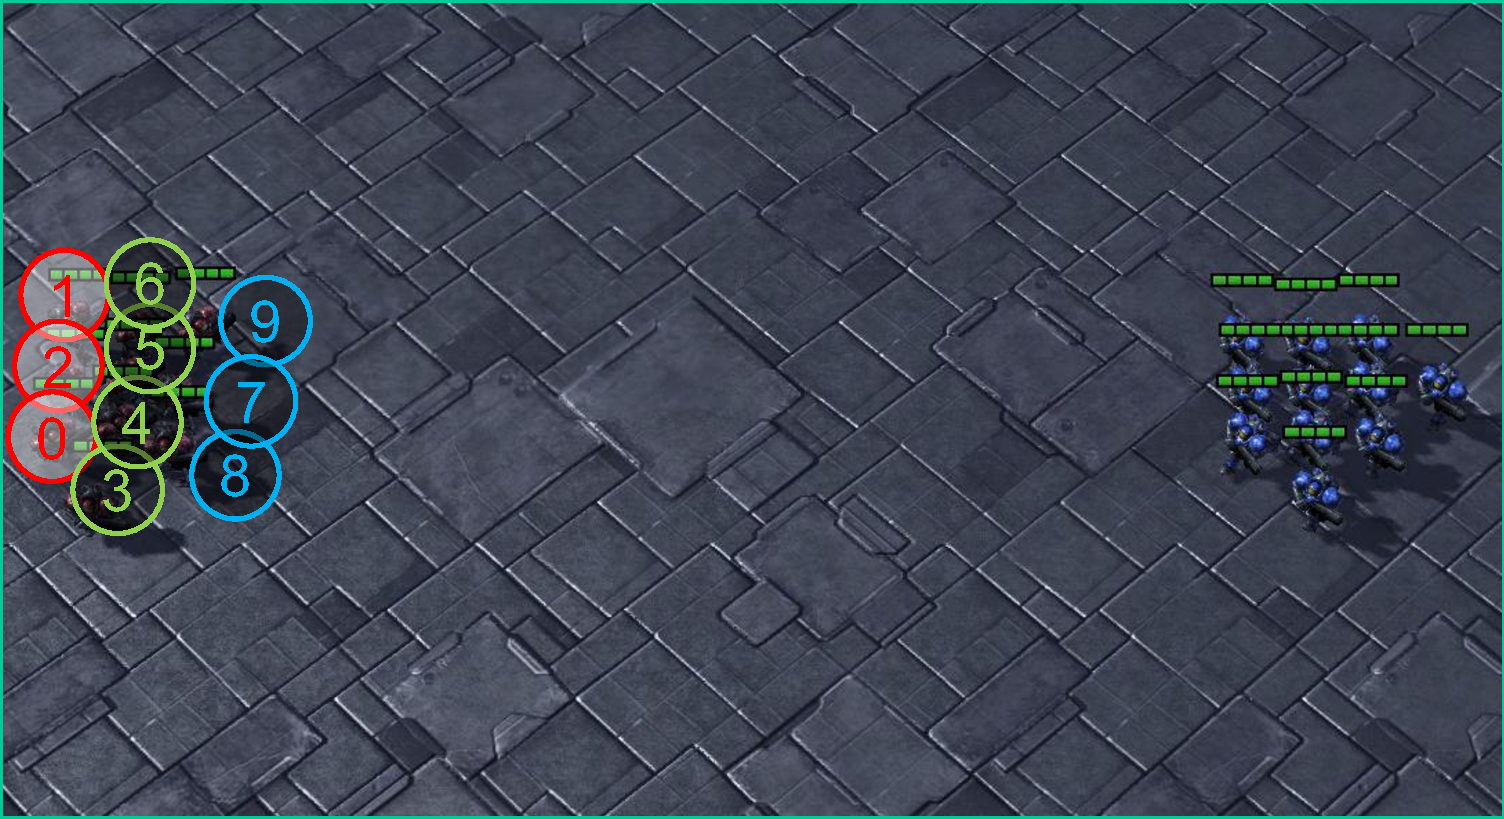
\includegraphics[height=0.17\linewidth]{img/fig-dynamic_roles/10m_vs_11m-g1.pdf}\hfill
            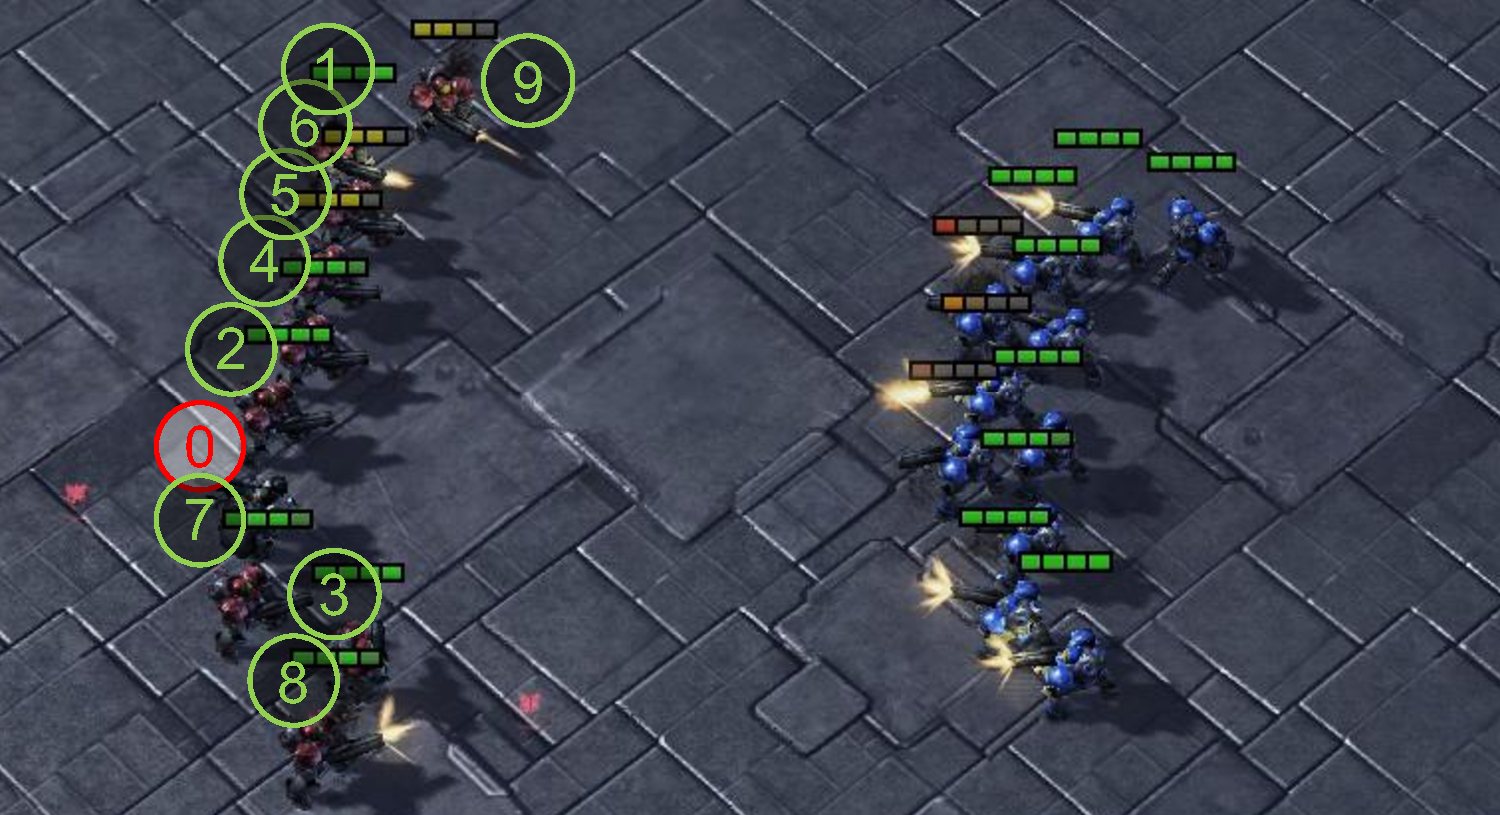
\includegraphics[height=0.17\linewidth]{img/fig-dynamic_roles/10m_vs_11m-g2.pdf}\hfill
            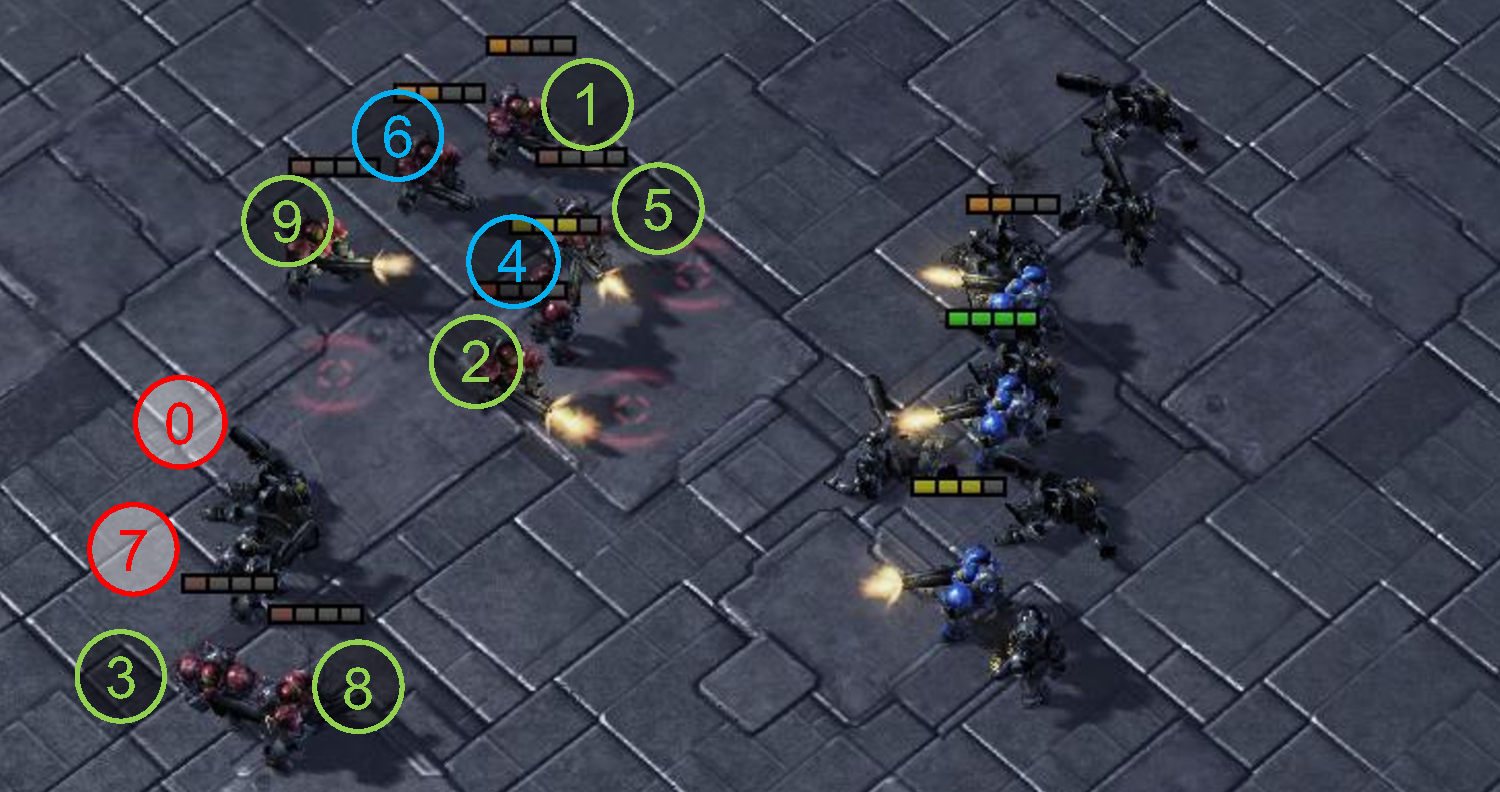
\includegraphics[height=0.17\linewidth]{img/fig-dynamic_roles/10m_vs_11m-g3.pdf}\\
            \subfigure[$t$=$1$]{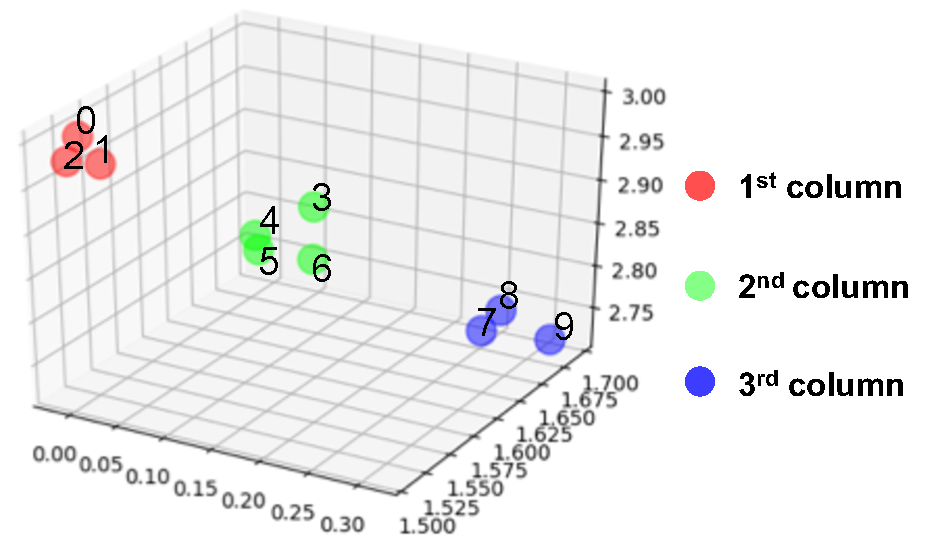
\includegraphics[width=0.32\linewidth]{img/fig-dynamic_roles/10m_vs_11m-r1-new.pdf}}\hfill
            \subfigure[$t$=$8$]{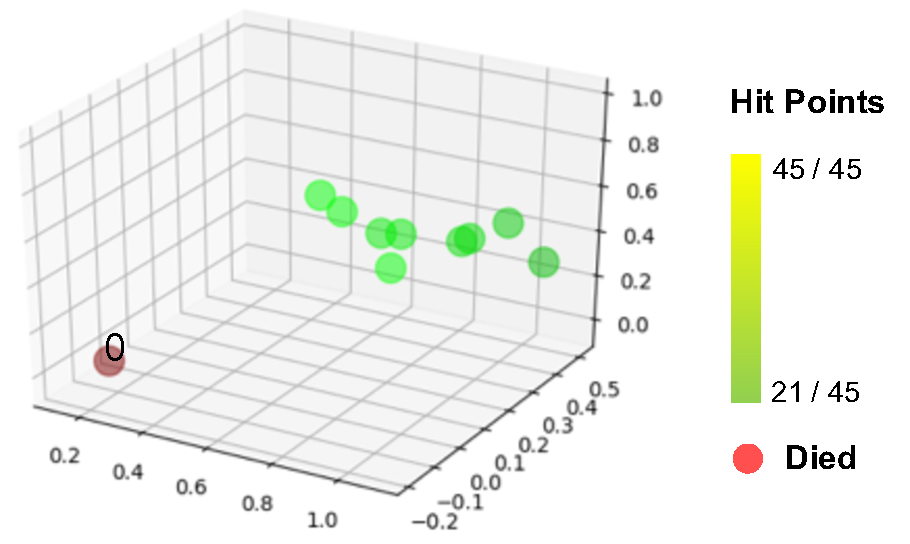
\includegraphics[width=0.32\linewidth]{img/fig-dynamic_roles/10m_vs_11m-r2-new.pdf}}\hfill
            \subfigure[$t$=$19$]{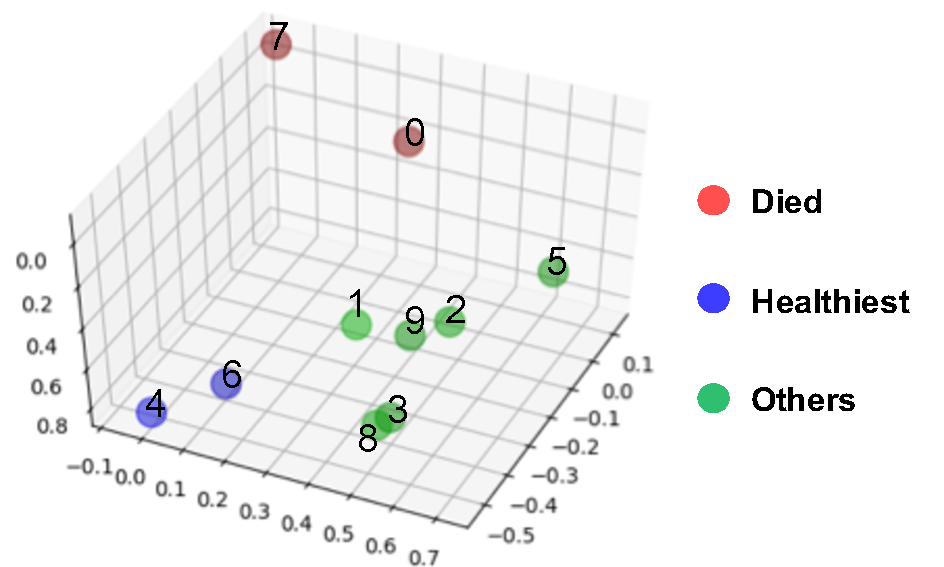
\includegraphics[width=0.32\linewidth]{img/fig-dynamic_roles/10m_vs_11m-r3-new.pdf}}
        \end{figure}
    \end{frame}

    \begin{frame}{Example of roles spaces}
        \begin{figure}
            \centering
            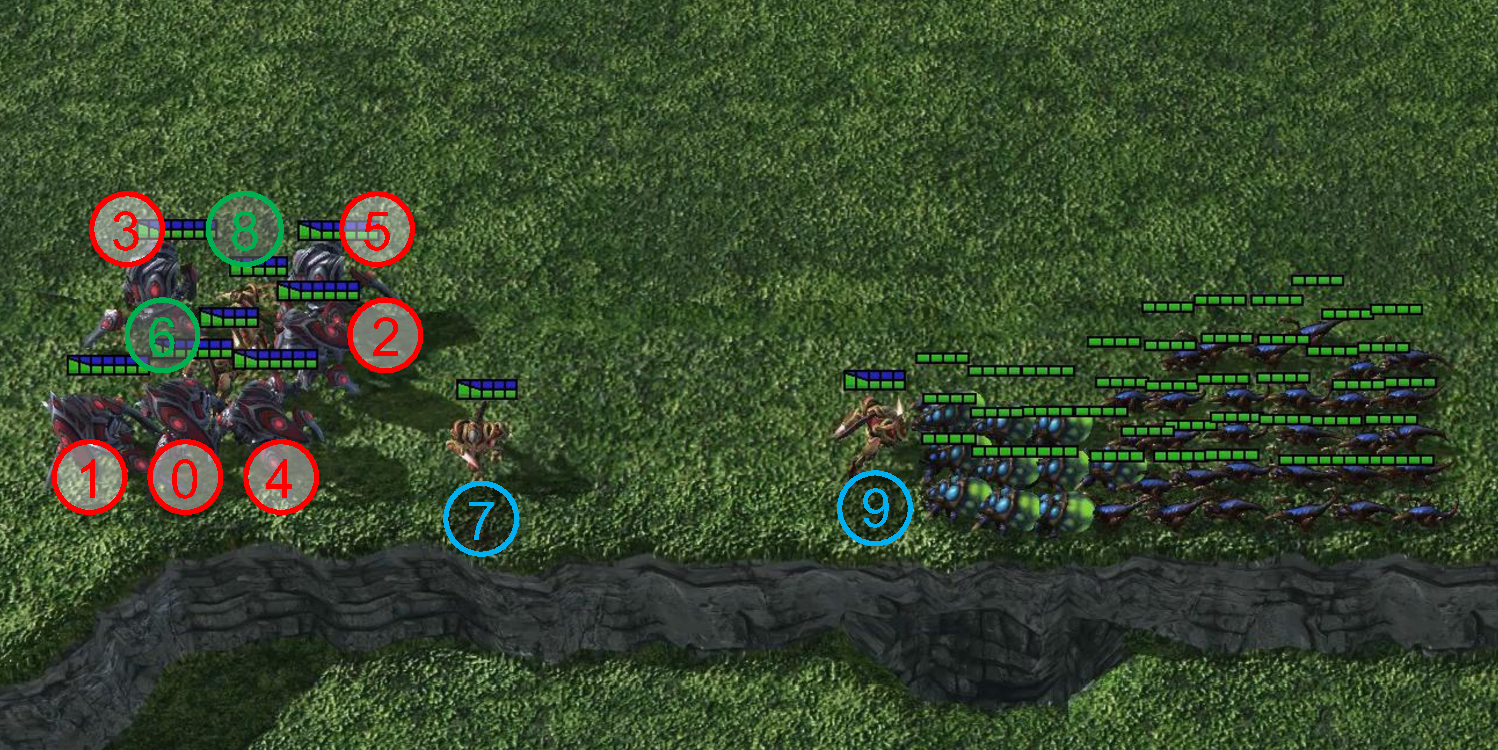
\includegraphics[width=0.32\linewidth]{img/fig-various_roles/various_roles-g1.pdf}\hfill
            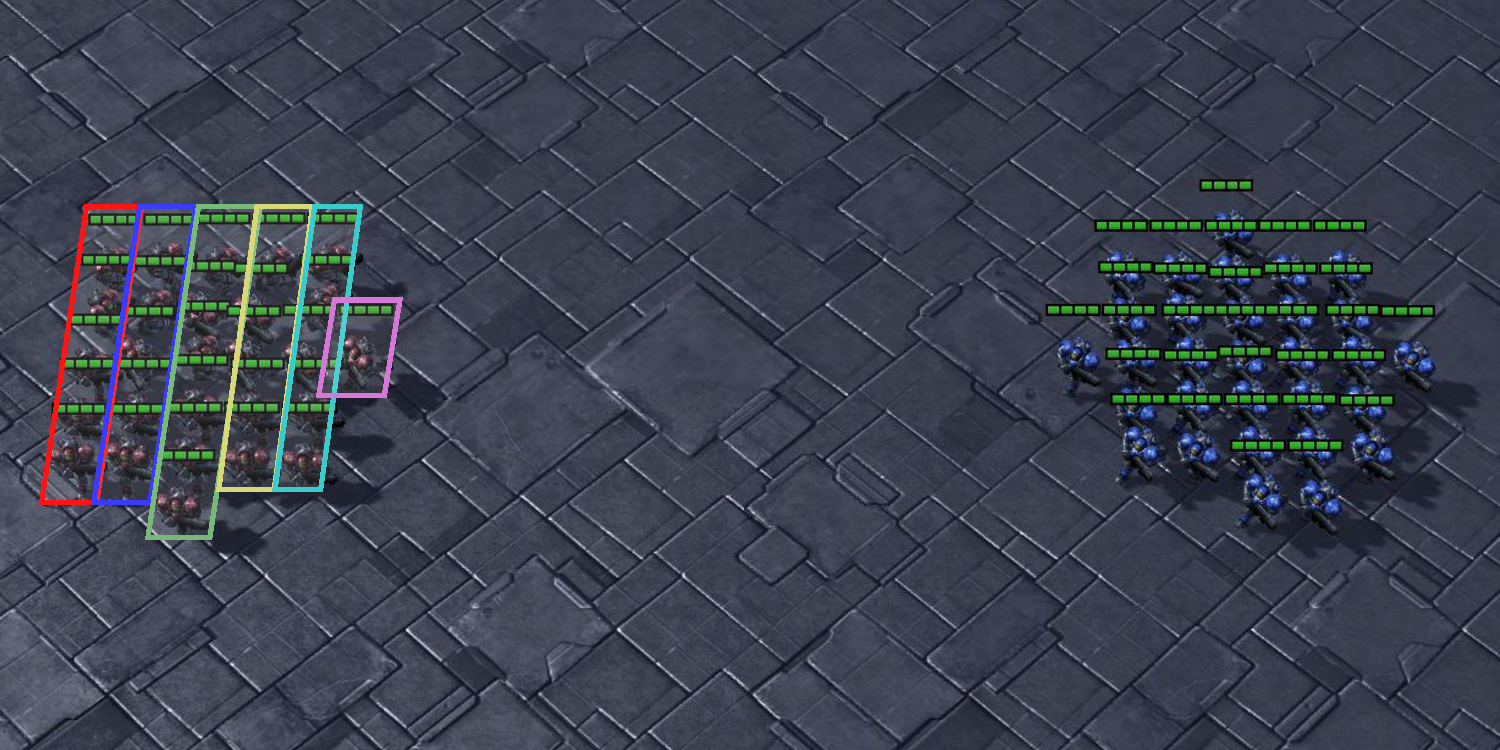
\includegraphics[width=0.32\linewidth]{img/fig-various_roles/various_roles-g2.pdf}\hfill
            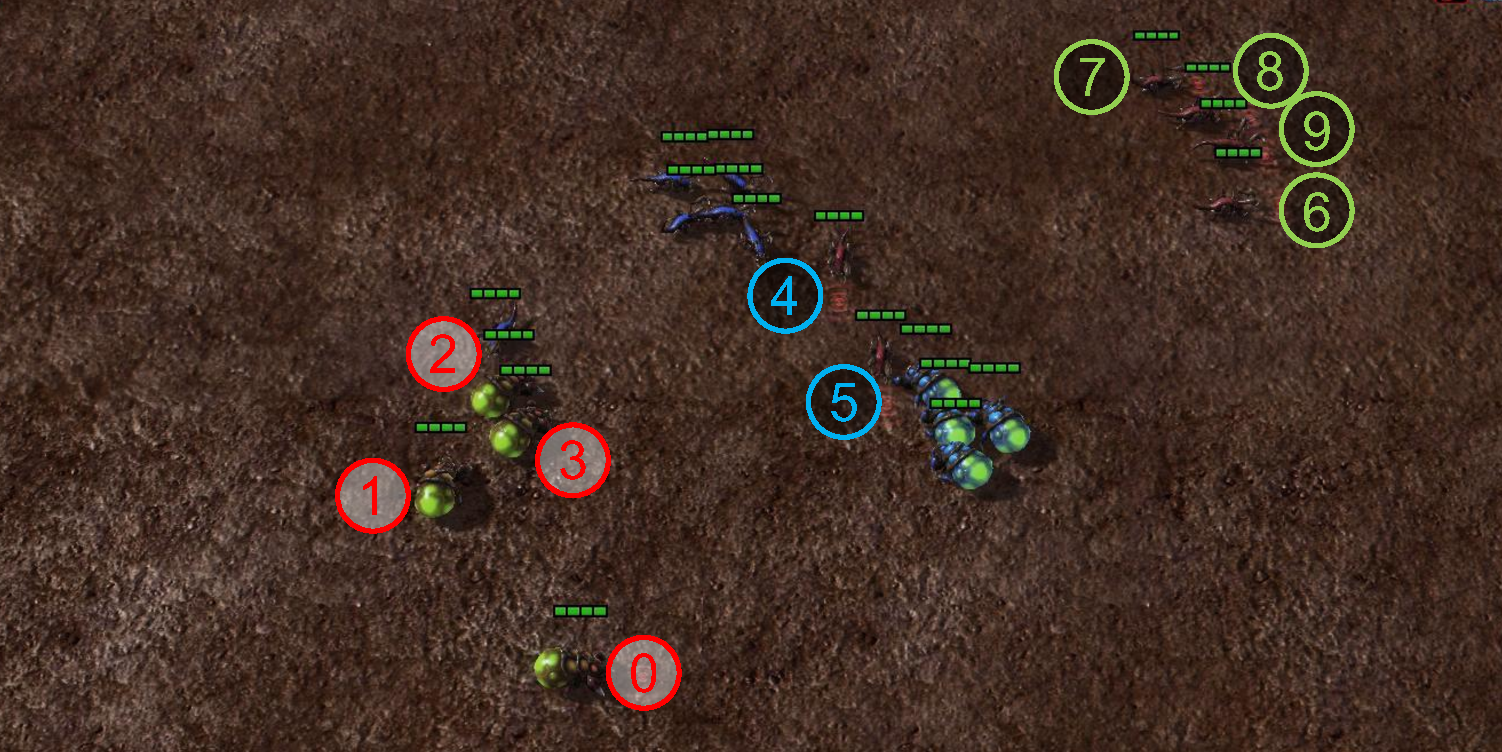
\includegraphics[width=0.32\linewidth]{img/fig-various_roles/various_roles-g3.pdf}
            \subfigure{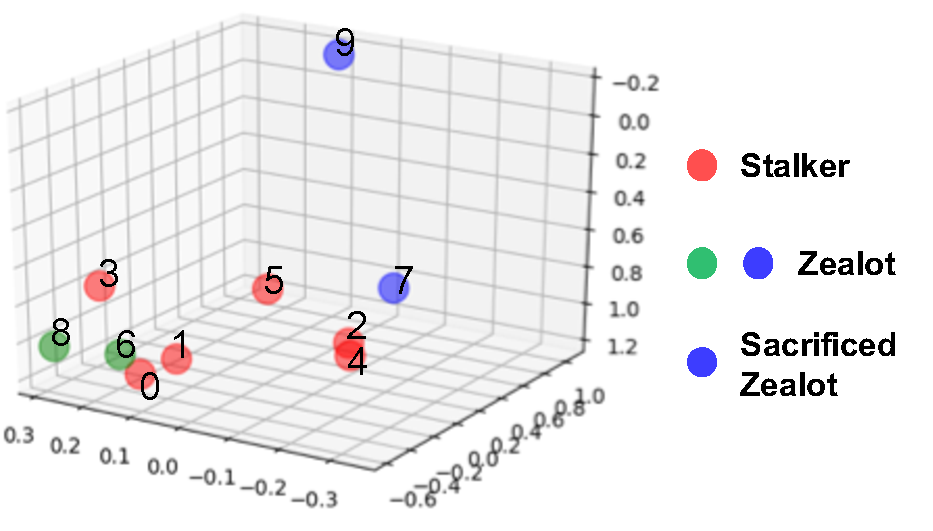
\includegraphics[width=0.32\linewidth]{img/fig-various_roles/various_roles-r1.pdf}\label{fig:various_roles-6s4z_vs_10b30z}}\hfill
            \subfigure{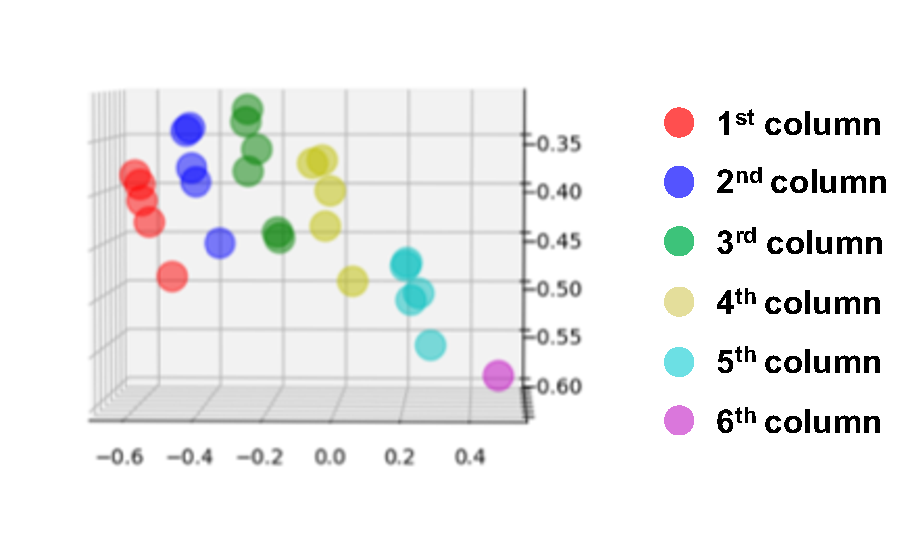
\includegraphics[width=0.32\linewidth]{img/fig-various_roles/various_roles-r2.pdf}}\hfill
            \subfigure{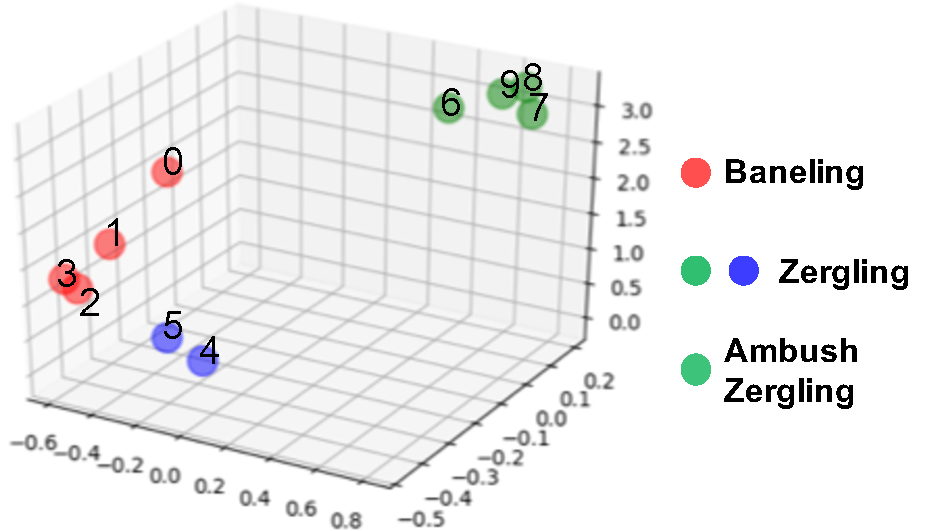
\includegraphics[width=0.32\linewidth]{img/fig-various_roles/various_roles-r3.pdf}}
        \end{figure}


    \end{frame}

    \begin{frame}{Conclusion}

        \begin{itemize}
            \item Improving the mixing architectures on complex hierachical tasks,
            \item by using a stochastic roles embedding space.
            \item Learned trough 2 regularizations:
            \begin{itemize}
                \item Versatily+Identifiability sub-loss;
                \item Specialization sub-loss.
            \end{itemize}

        \end{itemize}


    \end{frame}


\end{document}

